\documentclass[a4paper]{report} 
% Change "article" to "report" to get rid of page number on title page
\usepackage{amsmath,amsfonts,amsthm,amssymb}
% \numberwithin{equation}{section}

\usepackage{setspace}
\usepackage{fancyhdr}
\usepackage{lastpage}
\usepackage{extramarks}
\usepackage{chngpage}

\usepackage[usenames,dvipsnames]{color}

\usepackage{ifthen}
\usepackage{listings}
\usepackage{courier}


\usepackage[utf8]{inputenc}
\usepackage[english]{babel}


%% This are packages I'm using:
\usepackage{physics}
\usepackage{siunitx}
\usepackage{color}
\usepackage{hyperref}
\usepackage{cancel}
\usepackage[toc]{appendix}



\hypersetup{
    colorlinks=false, %set true if you want colored links
    linktoc=all,     %set to all if you want both sections and subsections linked
    linkcolor=blue,  %choose some color if you want links to stand out
}
\usepackage{graphicx}
\usepackage{subcaption}
\usepackage{dsfont}
\usepackage{mathrsfs}  


%   !!!!!!!!!!!!!!!!!!!!!!!!!!!!!!!!!!!!!!!!!!!!!!!!!!!!!
%
%   Name: Juan Antonio Fernández de la Garza
%   Due date: ------------------
%	Title: Proseminar report: Quantum gauge theory simulation
%
%   !!!!!!!!!!!!!!!!!!!!!!!!!!!!!!!!!!!!!!!!!!!!!!!!!!!!!


% Homework Specific Information
\newcommand{\hmwkTitle}{Simulations of lattice gauge theories}
\newcommand{\hmwkSubTitle}{}
\newcommand{\hmwkDueDate}{April 11, 2022}
\newcommand{\hmwkClass}{MSc Proseminar \\ ``Quantum Information: From Foundations to Algorithms"}
\newcommand{\hmwkClassTime}{}
\newcommand{\hmwkClassInstructor}{Dr. Joao Pinto Barros}
\newcommand{\hmwkAuthorNameI}{Juan Fernandez de la Garza}
\newcommand{\hmwkAuthorSCIPER}{}
%
%

% In case you need to adjust margins:
\topmargin=-0.45in      %
\evensidemargin=0in     %
\oddsidemargin=0in      %
\textwidth=6.5in        %
\textheight=9.5in       %
\headsep=0.25in         %

% This is the color used for  comments below
\definecolor{MyDarkGreen}{rgb}{0.0,0.4,0.0}

% For faster processing, load Matlab syntax for listings
\lstloadlanguages{Matlab}%
\lstset{language=Matlab,                        % Use MATLAB
        frame=single,                           % Single frame around code
        basicstyle=\small\ttfamily,             % Use small true type font
        keywordstyle=[1]\color{Blue}\bf,        % MATLAB functions bold and blue
        keywordstyle=[2]\color{Purple},         % MATLAB function arguments purple
        keywordstyle=[3]\color{Blue}\underbar,  % User functions underlined and blue
        identifierstyle=,                       % Nothing special about identifiers
                                                % Comments small dark green courier
        commentstyle=\usefont{T1}{pcr}{m}{sl}\color{MyDarkGreen}\small,
        stringstyle=\color{Purple},             % Strings are purple
        showstringspaces=false,                 % Don't put marks in string spaces
        tabsize=3,                              % 5 spaces per tab
        %
        %%% Put standard MATLAB functions not included in the default
        %%% language here
        morekeywords={xlim,ylim,var,alpha,factorial,poissrnd,normpdf,normcdf},
        %
        %%% Put MATLAB function parameters here
        morekeywords=[2]{on, off, interp},
        %
        %%% Put user defined functions here
        morekeywords=[3]{FindESS, homework_example},
        %
        morecomment=[l][\color{Blue}]{...},     % Line continuation (...) like blue comment
        numbers=left,                           % Line numbers on left
        firstnumber=1,                          % Line numbers start with line 1
        numberstyle=\tiny\color{Blue},          % Line numbers are blue
        stepnumber=1                        % Line numbers go in steps of 5
        }

% Setup the header and footer
\pagestyle{fancy}                                                       %
% \lhead{\hmwkAuthorName \quad \hmwkAuthorSCIPER}                       
\lhead{}
%\chead{\hmwkClass\ (\hmwkClassInstructor\ \hmwkClassTime): \hmwkTitle}  %
\rhead{\hmwkClass}  %
%\rhead{\firstxmark}                                                     %
\lfoot{\lastxmark}                                                      %
\cfoot{}                                                                %
\rfoot{Page\ \thepage\ out of\ \protect\pageref{LastPage}}                  %
\renewcommand\headrulewidth{0.4pt}                                      %
\renewcommand\footrulewidth{0.4pt}                                      %

% This is used to trace down (pinpoint) problems
% in latex a document:
%\tracingall

%%%%%%%%%%%%%%%%%%%%%%%%%%%%%%%%%%%%%%%%%%%%%%%%%%%%%%%%%%%%%
% Some tools
\newcommand{\enterProblemHeader}[1]{\nobreak\extramarks{#1}{#1 continued on next page\ldots}\nobreak%
                                    \nobreak\extramarks{#1 (continued)}{#1 continued on next page\ldots}\nobreak}%
\newcommand{\exitProblemHeader}[1]{\nobreak\extramarks{#1 (continued)}{#1 continued on next page\ldots}\nobreak%
                                   \nobreak\extramarks{#1}{}\nobreak}%

\newlength{\labelLength}
\newcommand{\labelAnswer}[2]
  {\settowidth{\labelLength}{#1}%
   \addtolength{\labelLength}{0.25in}%
   \changetext{}{-\labelLength}{}{}{}%
   \noindent\fbox{\begin{minipage}[c]{\columnwidth}#2\end{minipage}}%
   \marginpar{\fbox{#1}}%

   % We put the blank space above in order to make sure this
   % \marginpar gets correctly placed.
   \changetext{}{+\labelLength}{}{}{}}%

\setcounter{secnumdepth}{0}
\newcommand{\homeworkProblemName}{}%
\newcounter{homeworkProblemCounter}%
\newenvironment{homeworkProblem}[1][Problem \arabic{homeworkProblemCounter}]%
  {\stepcounter{homeworkProblemCounter}%
   \renewcommand{\homeworkProblemName}{#1}%
   \section{\homeworkProblemName}%
   \enterProblemHeader{\homeworkProblemName}}%
  {\exitProblemHeader{\homeworkProblemName}}%

\newcommand{\problemAnswer}[1]
  {\noindent\fbox{\begin{minipage}[c]{\columnwidth}#1\end{minipage}}}%

\newcommand{\problemLAnswer}[1]
  {\labelAnswer{\homeworkProblemName}{#1}}

\newcommand{\homeworkSectionName}{}%
\newlength{\homeworkSectionLabelLength}{}%
\newenvironment{homeworkSection}[1]%
  {% We put this space here to make sure we're not connected to the above.
   % Otherwise the changetext can do funny things to the other margin

   \renewcommand{\homeworkSectionName}{#1}%
   \settowidth{\homeworkSectionLabelLength}{\homeworkSectionName}%
   \addtolength{\homeworkSectionLabelLength}{0.25in}%
   \changetext{}{-\homeworkSectionLabelLength}{}{}{}%
   \subsection{\homeworkSectionName}%
   \enterProblemHeader{\homeworkProblemName\ [\homeworkSectionName]}}%
  {\enterProblemHeader{\homeworkProblemName}%

   % We put the blank space above in order to make sure this margin
   % change doesn't happen too soon (otherwise \sectionAnswer's can
   % get ugly about their \marginpar placement.
   \changetext{}{+\homeworkSectionLabelLength}{}{}{}}%

\newcommand{\sectionAnswer}[1]
  {% We put this space here to make sure we're disconnected from the previous
   % passage

   \noindent\fbox{\begin{minipage}[c]{\columnwidth}#1\end{minipage}}%
   \enterProblemHeader{\homeworkProblemName}\exitProblemHeader{\homeworkProblemName}%
   \marginpar{\fbox{\homeworkSectionName}}%

   % We put the blank space above to make sure this
   % \marginpar gets correctly placed.
   }%

%%% I think \captionwidth (commented out below) can go away
%%%
%% Edits the caption width
%\newcommand{\captionwidth}[1]{%
%  \dimen0=\columnwidth   \advance\dimen0 by-#1\relax
%  \divide\dimen0 by2
%  \advance\leftskip by\dimen0
%  \advance\rightskip by\dimen0
%}

% Includes a figure
% The first parameter is the label, which is also the name of the figure
%   with or without the extension (e.g., .eps, .fig, .png, .gif, etc.)
%   IF NO EXTENSION IS GIVEN, LaTeX will look for the most appropriate one.
%   This means that if a DVI (or PS) is being produced, it will look for
%   an eps. If a PDF is being produced, it will look for nearly anything
%   else (gif, jpg, png, et cetera). Because of this, when I generate figures
%   I typically generate an eps and a png to allow me the most flexibility
%   when rendering my document.
% The second parameter is the width of the figure normalized to column width
%   (e.g. 0.5 for half a column, 0.75 for 75% of the column)
% The third parameter is the caption.
\newcommand{\scalefig}[3]{
  \begin{figure}[ht!]
    % Requires \usepackage{graphicx}
    \centering
    \includegraphics[width=#2\columnwidth]{#1}
    %%% I think \captionwidth (see above) can go away as long as
    %%% \centering is above
    %\captionwidth{#2\columnwidth}%
    \caption{#3}
    \label{#1}
  \end{figure}}

% Includes a MATLAB script.
% The first parameter is the label, which also is the name of the script
%   without the .m.
% The second parameter is the optional caption.
\newcommand{\matlabscript}[2]
  {\begin{itemize}\item[]\lstinputlisting[caption=#2,label=#1]{#1.m}\end{itemize}}

%%%%%%%%%%%%%%%%%%%%%%%%%%%%%%%%%%%%%%%%%%%%%%%%%%%%%%%%%%%%%


%%%%%%%%%%%%%%%%%%%%%%%%%%%%%%%%%%%%%%%%%%%%%%%%%%%%%%%%%%%%%
% Make title
%\title{\vspace{2in}\textmd{\textbf{\hmwkClass:\ \hmwkTitle\ifthenelse{\equal{\hmwkSubTitle}{}}{}{\\\hmwkSubTitle}}}\\\normalsize\vspace{0.1in}\small{Due\ on\ \hmwkDueDate}\\\vspace{0.1in}\large{\textit{\hmwkClassInstructor\ \hmwkClassTime}}\vspace{3in}}
\title{\vspace{1in}\textmd{\textbf{\hmwkClass: \\ \hmwkTitle\ifthenelse{\equal{\hmwkSubTitle}{}}{}{\\\hmwkSubTitle}}}\\\normalsize\vspace{0.1in}\small{\hmwkDueDate}\\\vspace{0.5in}
\includegraphics[width=0.4\linewidth]{logo.png}\\\large{\textit{ \hmwkClassTime}}\vspace{2in}}
\date{}


\author{\textbf{\hmwkAuthorNameI}}% \\ \\ Tutor: \\ \textbf{\hmwkClassInstructor}  \\ \\    \\ \\ }
%%%%%%%%%%%%%%%%%%%%%%%%%%%%%%%%%%%%%%%%%%%%%%%%%%%%%%%%%%%%%

\begin{document}
\begin{spacing}{1.1}

% \newpage

\maketitle
% \newpage
% \begin{figure}[h!]
%     \centering
%     
\includegraphics[width=0.4\linewidth]{logo.png}
%     \label{fig:my_label}
% \end{figure}% Table des matieres


% Uncomment the \tableofcontents and \newpage lines to get a Contents page
% Uncomment the \setcounter line as well if you do NOT want subsections
%       listed in Contents
\setcounter{tocdepth}{2}
\tableofcontents
\newpage





% When problems are long, it may be desirable to put a \newpage or a
% \clearpage before each homeworkProblem environment

%\newpage


%%%%%%%%%%%%%%%%%%%%%%%%%%%%%%%%%%%%%%%%%%%%%%%%%%%%%%%%%%%%%

\section{Introduction} 

This report contains a general overview of simulations of lattice gauge theories to discuss a theoretical setting that allows for quantum simulations. It will start by presenting Wilson's formalism, then apply it to define Wilson's Hamiltonian of quantum electrodynamics (QED). Afterwards, quantum link models are introduced and used to state a Hamiltonian for lattice quantum electrodynamics ($U(1)$ gauge symmetry) and a Hamiltonian for a $SU(N)$ lattice gauge theory. A short discussion on the symmetric properties of both theories is also included, which allows an interpretation of the physically realizable quantum states, based on the generators of the symmetry in each theory.

% Through the report, the lattice systems are classified in terms of their dimensions. For clarification purposes, whenever we have a $(d+1)$ dimensional Hamiltonian system, 

% a summary of the two gauge theories that are relevant/popular in physics: with U(1), and SU(3) local gauge symmetries, which correspond to QED and QCD. Then, a discussion on the generators of each theory, and relevant relationships that allows us to write these theories making use of a lattice Hamiltonian which is to be taken to the continuum. 

Finally, a discussion is included on how fermionic and bosonic quantum operators can be transformed into spin operators. In particular, an example of this with a quantum link model of QED is discussed. 

% the main objective of this report is to show how a gauge theory can be defined on a spin-lattice, which can then be simulated with a quantum computer.???

% include remark on the spacetime dimensions and how they are related to the way the theories are quantized.
% d+1 Lagrangian -> d+1 discrete dims
% d+1 Hamiltonian -> d discrete + time cont.


% \textit{Last update: April 3, 2022.}



\section{Lattice gauge theories}

A lattice gauge theory corresponds to a physical system that lives on a lattice, where its dynamics are invariant upon local (gauge) transformations. These transformations form a symmetry group (also called gauge group), and the symmetry group has its set of generators, which can be used to construct a general gauge transformation belonging to the symmetry group. For the case of continuous symmetries, the symmetry groups are Lie groups, which can be Abelian (e.g. $U(1)$) or non-Abelian (e.g. $SU(N)$).

Two main gauge theories will be discussed throughout this report. One of which is QED, which is a theory with $U(1)$ gauge symmetry, so the symmetry has 1 generator. This generator corresponds to one bosonic degree of freedom, which in QED becomes the photon and mediates the interactions between spin$-1/2$ particles and antiparticles with an electric charge.

The other relevant gauge theory for this report is the one with $SU(N)$ gauge symmetry. This symmetry has $N^2-1$) generators. A physical example is QCD, which is a theory with $SU(3)$ gauge symmetry, so it has 8 generators that correspond to 8 bosonic degrees of freedom, i.e. 8 gluons mediating strong interaction between quarks with color charge.




% we mainly discuss a physical system consisting of an (infinite) lattice that contains in its dynamics terms that can be interpreted to physical fields present in Gauge theories.

% Consider a field theory described by a Lagrangian. There are interesting cases in which the Lagrangian of the system is invariant concerning a specific set of continuous transformations of spacetime, which form a Lie group. This Lie group can be Abelian or Non-Abelian, referring to the nature of commutative properties of these transformations.

% These groups have generators and each generator corresponds to a degree of freedom.

% of one of these symmetries implies the existence of one gauge degree of freedom to the theory, that is nevertheless ``hidden" from the physical behavior, but allows us to define it to convenience and recover different physical interpretations of the same phenomena. In other words, the gauge freedom corresponds to a gauge field and thus the gauge is a formalism to regulate these freedoms that leave the Physics intact. 
% Furthermore, the fact that gauge symmetries exist, allows us to regularize and renormalize the theories such that we can do non-diverging calculations, so even if gauge freedoms look like innocent mathematical artifacts, they are fundamental for the physical understanding of field theories.

% In summary, Gauge transformations conform a Lie group, with a Lie algebra and generators of this group. Each generator then implies a vector field (gauge field), and upon a quantization procedure, the appearance of ``gauge bosons", more on that later on.

\subsection{A classical gauge symmetry}

A classical example where a gauge freedom seems physically irrelevant is in the case of classical electrodynamics, the equations that model this theory are Maxwell's equations:
\begin{align}
    \nabla \cdot E(t,\vb{x}) &= \rho(t,\vb{x}), \\
    \nabla \cdot B(t,\vb{x}) &= 0, \label{eq:ME2} \\
    \nabla \cross E(t,\vb{x}) + \partial_{t} B(t,\vb{x}) &= 0, \label{eq:ME3}\\
    \nabla \cross B(t,\vb{x}) - \partial_{t} E(t,\vb{x}) &= j(t,\vb{x}).
\end{align}
The electric and magnetic fields are physical observables (consider an experiment with a test charge where the electric and magnetic fields can be inferred). However, it is convenient to define electromagnetic potentials $\Phi(t,\vb{x}), \, \vb{A}(t,\vb{x})$ by considering
\begin{align}
    E &= - \nabla \Phi - \partial_t \vb{A}, \label{eq:Egauge}\\
    B &= \nabla \cross \vb{A},\label{eq:Mgauge}
\end{align}
which by construction implies that (\ref{eq:ME2}), (\ref{eq:ME3}) are solved. Nevertheless, this convenient choice is introducing ambiguity to the theory: there is now a local (gauge) transformation that leaves Maxwell's equations invariant.

The gauge transformation the following:
\begin{align}
    \vb{A}(t,\vb{x}) &\longmapsto \vb{A}(t,\vb{x}) - e\,\nabla\alpha(t,\vb{x}) \\
    \Phi(t,\vb{x}) &\longmapsto \Phi(t,\vb{x}) + e\,\partial_t \alpha(t,\vb{x}) 
\end{align}
(or with a covariant notation)
\begin{equation}
    A_\mu(x) \mapsto A'_\mu(x) = A_\mu(x) + e\,\partial_\mu \alpha(x),
\end{equation}
where $e$ is the electron charge and $A_\mu$ is the gauge field. From this result, notice that the gauge field in classical electrodynamics is made up of the vector potential and the electric potential.
%As seen in the next section, the gauge field $A_\mu(x)$ in classical electrodynamics transforms the same way as the photon field in QED.

Inserting this local transformation $\alpha(x)$ into (\ref{eq:Egauge}) and (\ref{eq:Mgauge}) via $(\Phi, \vb{A})$, the electric and magnetic fields are unaffected. Upon fixing the gauge by making a specific choice for $\alpha(x)$, the gauge redundancy is removed.

Although it seems that introducing the gauge field $A_\mu (x) $ is unnecessary for obtaining an accurate physical description, it is important to note that gauge fields are necessary when we go to the quantum context. In particular, in the path integral formulation, the electron interacts directly with the gauge field $A_\mu (x)$ through its Hamiltonian, and not via the electric and magnetic fields themselves. One relevant setup where the gauge field has observable physical consequences is when a thin solenoid with current is located in between the two slits of the double-slit experiment. The gauge field due to this thin solenoid implies a phase difference in the wave-function of an electron going through one slit or the other. This phase difference is $\Delta \phi = e \oint \vb{A}\cdot \dd \vb{x}$ and it implies a shift in the interference pattern the electron produces (view Figure \ref{fig:ABeffect} for reference). This is known as the Aharonov-Bohm effect \cite{aharonov1959significance}, which has been confirmed experimentally \cite{batelaan2009aharonov}. 

% as a shift in the interference pattern that an electron produces in the double-slit experiment with a thin solenoid between the slits: the Aharonov-Bohm effect
\begin{figure}[h!]
\centering
\begin{subfigure}{0.6\textwidth}
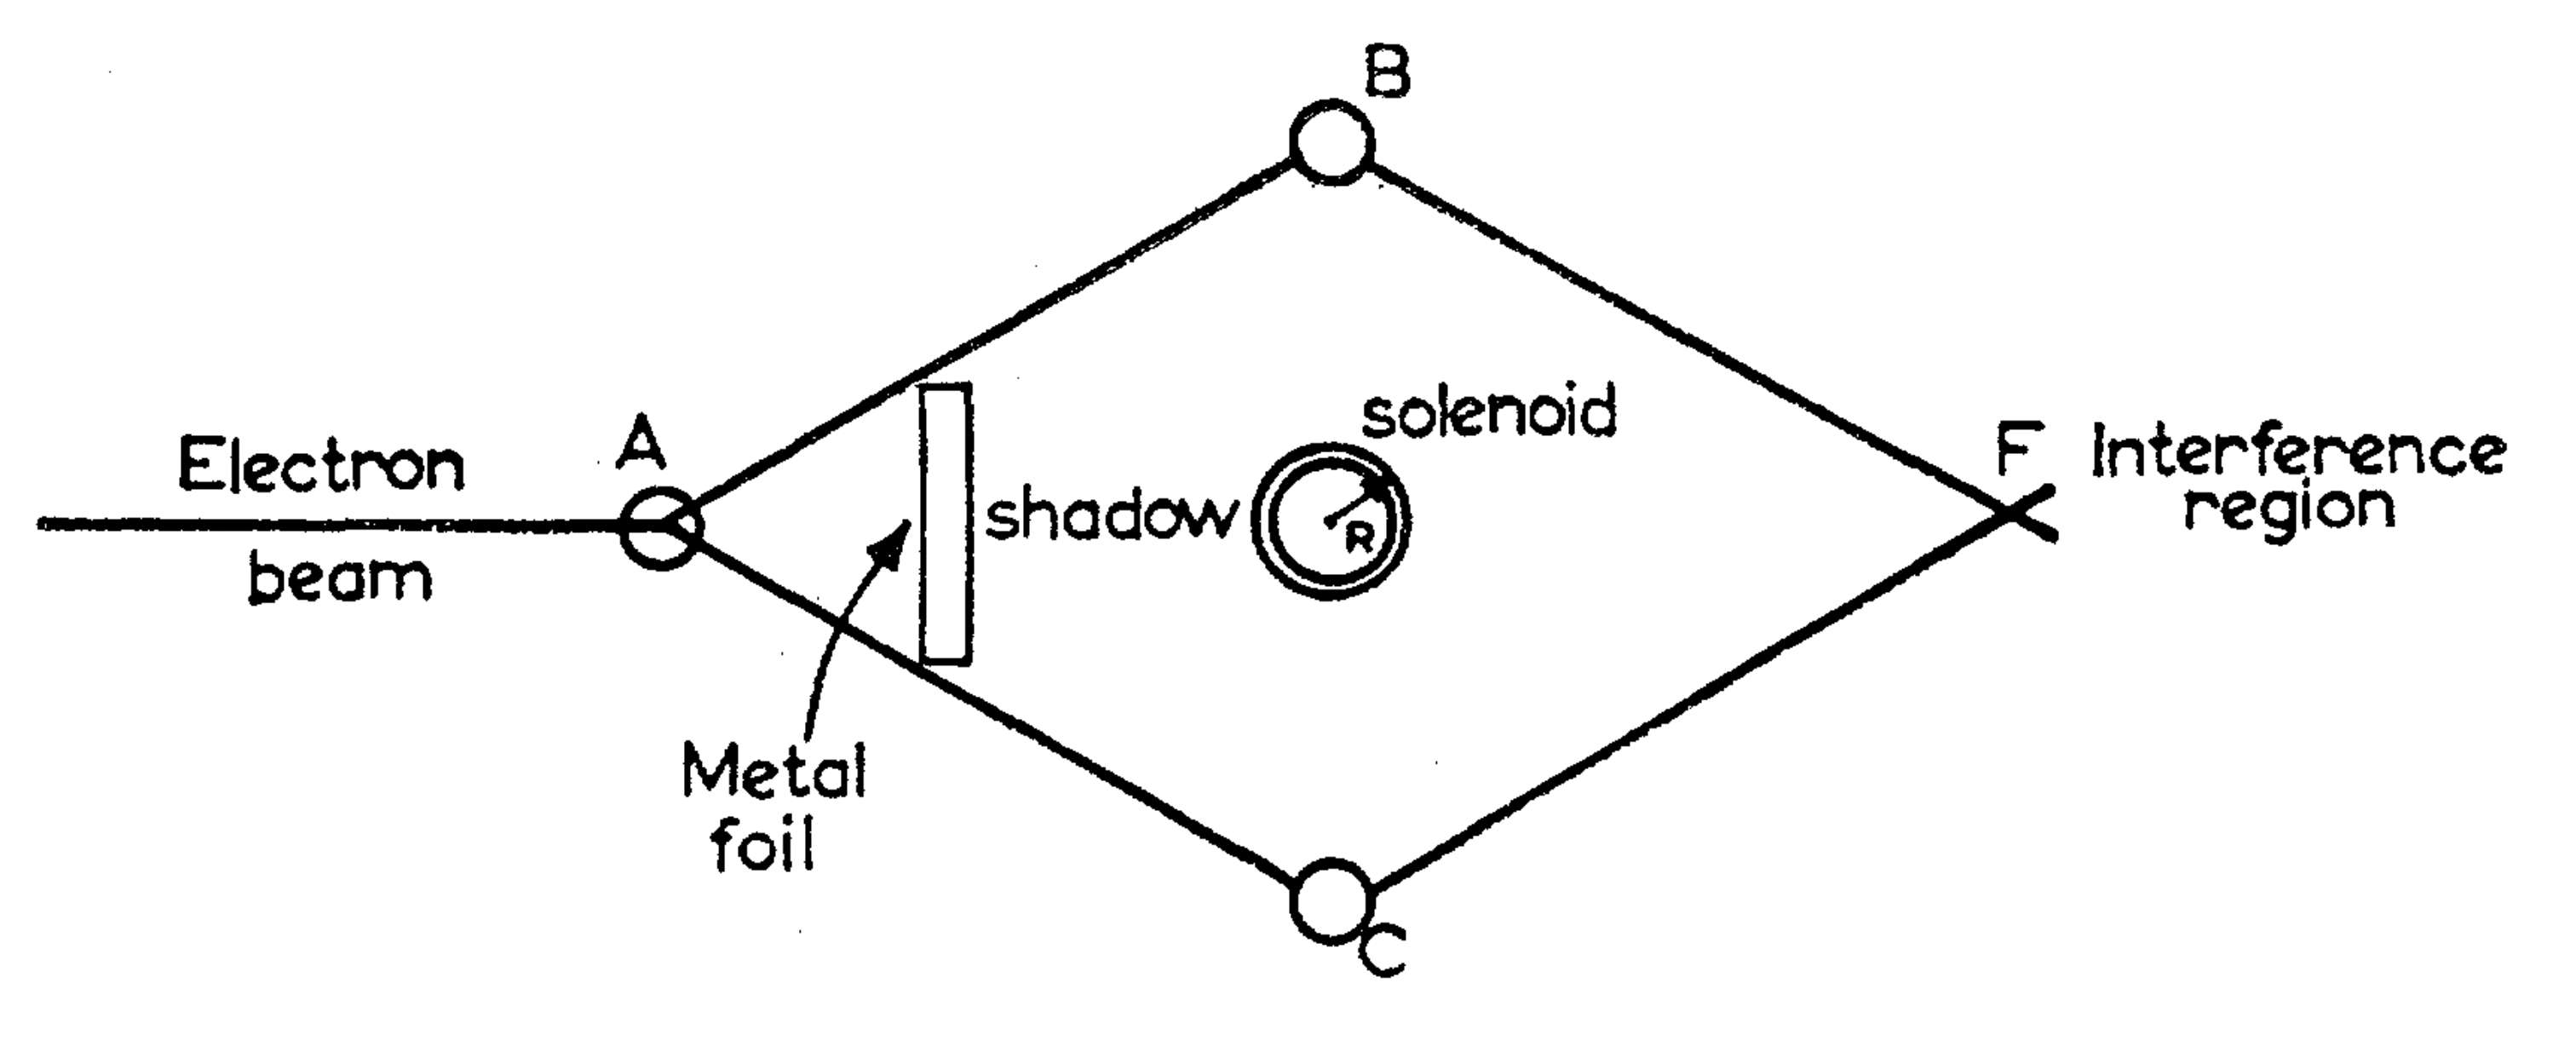
\includegraphics[width=\linewidth]{ABeffect.png} % change jpg to pdf when doing the final compilation of the pdf
\end{subfigure}
\caption{Reproduction of the Aharonov-Bohm effect diagram from the original paper by Aharonov and Bohm in 1959 \cite{aharonov1959significance} \label{fig:ABeffect}}
\end{figure}



% \subsection{A somewhat more interesting (but naive) example}

% I have this example written down on paper but after thinking about it, maybe it is not relevant. The example basically corresponds to introducing a minimal coupling to the differential operators in Schrodinger's equation to try to show that the local gauge symmetry enters in the shape of a local gauge in the phase of the wavefunction, but maybe this is just unnecessary, also as we know, (SE) is not valid in the relativistic limit.


\subsection{The Dirac free electron and the photon field}

In the quantum relativistic context, wave functions do not describe point particles, but instead, particles are excitations of the underlying fields described by a quantum field theory. In particular, for the Dirac free electron, its dynamics are described by the Lagrangian density
\begin{equation}
    \mathcal{L} = \overline{\psi}(x)(i\cancel\partial - m)\psi(x),
\end{equation}
which has a global $U(1)$ symmetry that can be observed by doing the transformation
\begin{equation}
    \psi(x) \mapsto \psi'(x) = \exp(ie\alpha)\psi(x).
\end{equation}
Although here $\alpha$ is just a number, we want to see what would happen if $\alpha$ is a spacetime function $\alpha(x)$. In other words, what happens to the fields if we impose a local $U(1)$ symmetry?

Trying naively to transform the Lagrangian density, we find
\begin{equation}
    \psi(x) \mapsto \psi'(x) = \exp(ie\alpha(x))\psi(x),
\end{equation}
\begin{equation}
    \cancel\partial \psi(x) \mapsto e^{ie\alpha(x)} \cancel\partial \psi(x) + (\cancel\partial e^{ie\alpha(x)} ) \psi(x).
\end{equation}
So it is convenient to define a ``covariant derivative" that can absorb the extra terms, such that we can recover a gauge-invariant Lagrangian density. This covariant derivative can be defined in the simplest non-trivial case by adding a spacetime function $f_\mu(x)$
\begin{equation}
    D_\mu = \partial_\mu + f_\mu(x),
\end{equation}
subject to compliance with the local $U(1)$ symmetry
\begin{equation}
    \cancel{D}\psi \mapsto e^{ie\alpha}\cancel{D}\psi.
\end{equation}
This implies that we have
\begin{align}
    D_\mu'\psi' &= e^{ie\alpha(x)}D_\mu \psi(x), \\
    (\partial_\mu + f'_\mu(x))(e^{ie\alpha(x)} \psi(x))&= e^{ie\alpha(x)} (\partial_\mu +f_\mu(x))\psi(x), \\
    (\partial_\mu e^{ie\alpha(x)})\psi(x) + f'_\mu(x) e^{ie\alpha(x)}\psi(x) &= f_\mu(x)e^{ie\alpha(x)}\psi(x), \\
    f'_\mu(x) \psi(x) &= (f_\mu(x) - ie\partial_\mu \alpha(x)) \psi(x),
\end{align}
or in other words, that the extra field $f_\mu(x)$ has to transform like
\begin{align}
    f_\mu(x) \mapsto f'_\mu(x) &= f_\mu(x) - ie\,\partial_\mu \alpha(x).
\end{align}
By doing a re-scaling as $i f_\mu(x) = A_\mu(x)$, our gauge field in QED transforms like the gauge field from classical electrodynamics:
\begin{equation}
    A_\mu(x) \mapsto A'_\mu(x) = A_\mu(x) + e\,\partial_\mu \alpha(x).
\end{equation}
Given that now the gauge theory is quantum, the gauge field corresponds to the photon field.

% By taking Dirac's free Action, and imposing a continuous local $U(1)$ symmetry in the Lagrangian density, we find that we need to couple the photon field through the covariant derivative (electron-photon interaction). 

To complete the gauge theory, the photon field dynamics are added via the field tensor $F_{\mu\nu} = \partial_\mu A_\nu - \partial_\nu A_\mu$, to define the Lagrangian density for QED:
\begin{equation} \label{eq:L_QED}
    \mathcal{L} = \overline{\psi}(i\,\cancel D-m)\psi-\frac{1}{4}F_{\mu\nu}F^{\mu\nu}.
\end{equation}

% , on which electrons and positrons appear as excitations and become coupled (and interact) via the electromagnetic photon field.

% And as any self-interacting field, we encountered divergences that have to be corrected via regularization and renormalization techniques.
% x

\section{Defining the lattice}

In a quantum field theory, scattering amplitudes are expectation values of the interactions between the particles involved in the theory. However, we often encounter that the integrals of these expectation values contain divergences that are systematically removed by renormalizing the theory, such that now the scattering amplitudes are finite and correspond to the experimentally observable values. One way to renormalize a theory is by introducing momentum cutoffs.

On the other hand, it is possible to define a gauge theory in a lattice and simulate this with computational methods to obtain numerical estimates of these scattering amplitudes. When properly discretized, the lattice gauge theory reproduces the continuous gauge theory when the lattice spacing $a\xrightarrow[]{}0$. Furthermore, defining a lattice theory introduces a natural momentum cutoff $\sim 1/a$, because the interaction length-scale is at least the size of the lattice spacing; so the regularization of a quantum field theory can be done via the lattice parameters \cite{wiese2013ultracold}.

% With this in mind, we can set our goal for today: introduce a lattice that encodes a Gauge Theory, and send $a \xrightarrow[]{} 0$ in a systematic and sensible way to obtain the continuous limit of a Gauge theory in a lattice.



\subsection{A staggered lattice}

There is not a unique way of defining a lattice gauge theory. For example, two distinct lattice gauge theories correspond to different physical systems, but as long as in the continuous limit ($a\xrightarrow[]{}0$) both converge to the same continuous gauge theory, they represent the same quantum field theory\footnote{Converging to the same continuous gauge theory means obtaining the same \textbf{long-distance} physics.} \cite{wiese2013ultracold,dalmonte2016lattice}.

One possible lattice definition consists of staggering particle-antiparticle fermionic sites in the lattice (a checkered pattern). In the case of Dirac's electron, this can be useful because we separate the spin-dependence (particle-antiparticle representation) from the fermionic fields, and instead the spin is incorporated by staggering particle and antiparticle sites in the lattice \cite{wiese2013ultracold}.

% For example, the particle and anti-particle representation in a 2D lattice with a checkered pattern (like in Dalmonte's Review). This results in a spin-less fermionic system from the Condensed Matter Physics point of view

% INTRODUCE A DIAGRAM OF THE LATTICE SETUP 
\begin{figure}[h!]
\centering
\begin{subfigure}{0.4\textwidth}
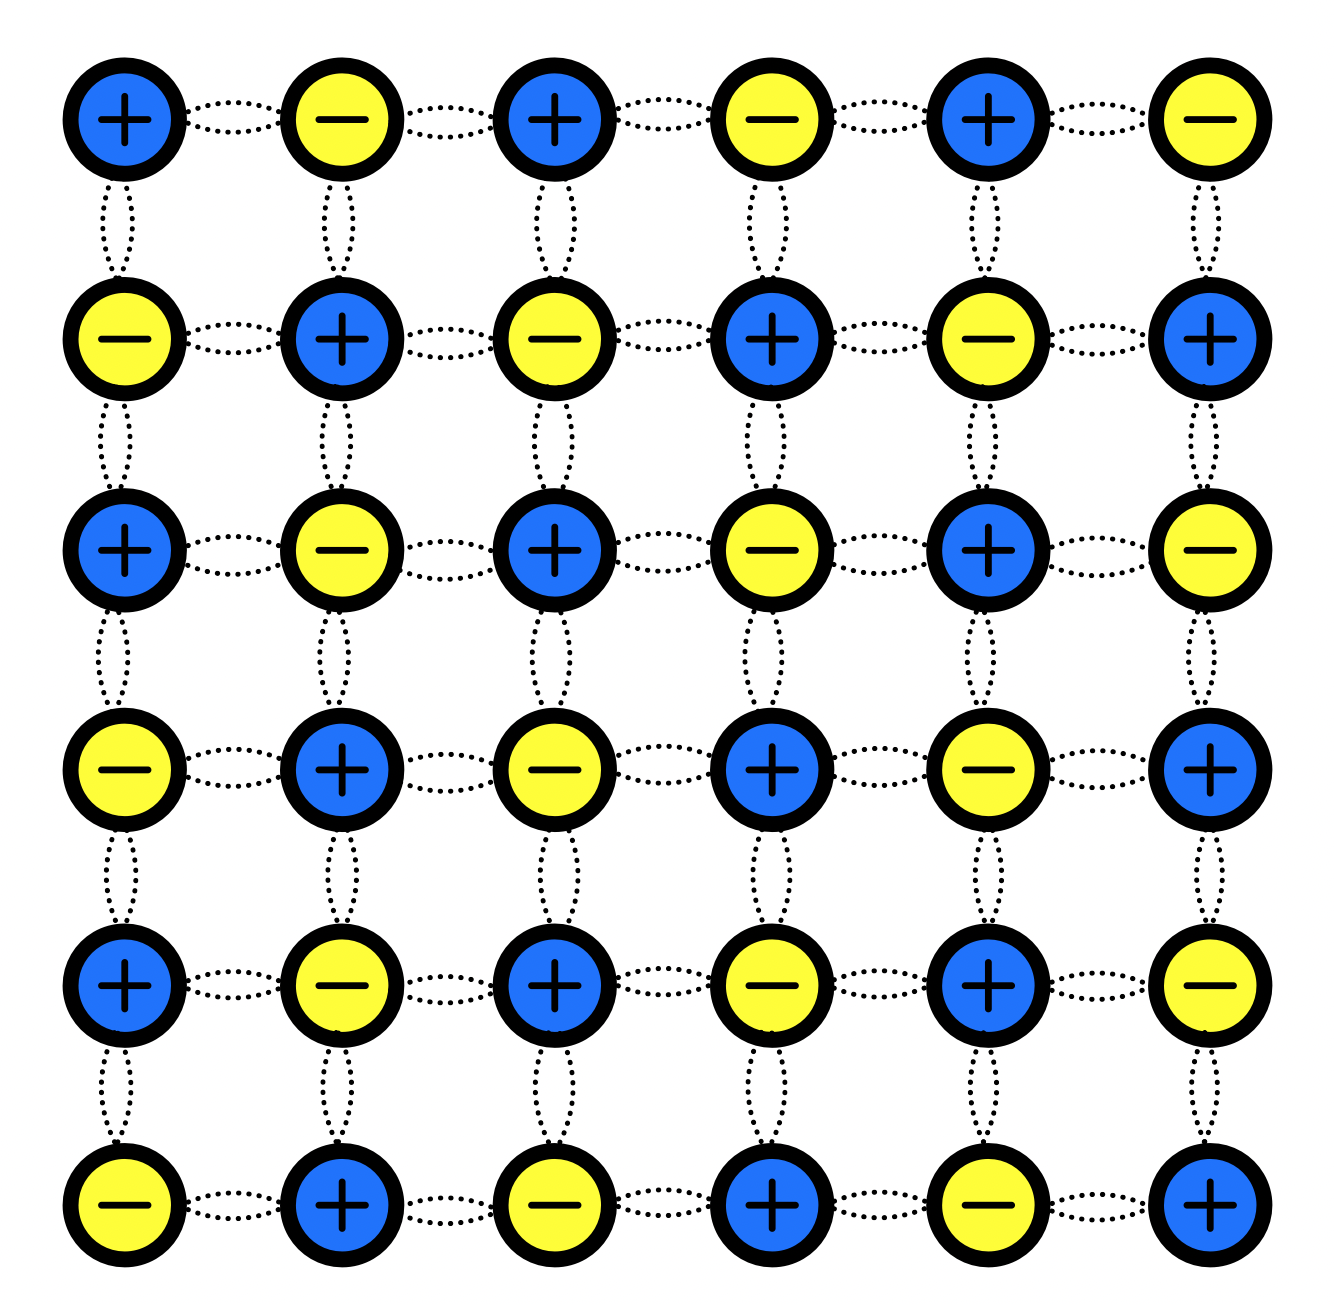
\includegraphics[width=\linewidth]{StaggeredLat.png} % change jpg to pdf when doing the final compilation of the pdf
\end{subfigure}
\caption{Pictorial view of what the staggered lattice looks like for a square lattice. The blue ($+$) sites represent fermion particles and the yellow ($-$) sites represent fermion anti-particles.}
\end{figure}


For the free Dirac's free electron, we can define a discrete version of the Lagrangian in a lattice as follows. Starting from the Lagrangian definition
\begin{equation}
    S = \int \dd^d x\, \overline{\psi}(x) ( i \gamma_{\mu} \partial^{\mu} - m) \psi(x),
\end{equation}
we can apply a finite differences scheme to perform a discrete derivative
\begin{equation}
    \partial^{\mu} \psi(x) \mapsto \frac{1}{2a} \left[\psi(x+k^{\mu} a) - \psi(x-k^{\mu} a) \right] \equiv \frac{1}{2a} \left(\psi_{x+\mu} - \psi_{x-\mu} \right),
\end{equation}
\begin{equation} \label{eq:SQED}
    \implies \int \dd^d x\, \overline{\psi}(x) ( i \gamma_{\mu} \partial^{\mu} - m) \psi(x) \mapsto \sum_{x,\mu} a^d \left[ \overline{\psi}_x \frac{i \gamma_{\mu} }{2a} \psi_{x+\mu} - \overline{\psi}_x \frac{i \gamma_{\mu} }{2a} \psi_{x-\mu} - m \overline{\psi}_x\psi_x \right],
\end{equation}
where $d$ refers to the number of space-time dimensions in the lattice system, and $\mu$ indexes these dimensions. $\gamma^\mu$ are the elements of Dirac's algebra ($\{\gamma^\mu \gamma^\nu \} = 2 g^{\mu\nu} \mathds{1}$) for $g^{\mu\nu}$ being the metric. In principle, a discretized Lagrangian density can be defined and used to perform computational simulations on a lattice. For clarification purposes, a $d$-dimensional lattice in the Lagrangian formalism is made up of $d-1$ discrete spatial dimensions and $1$ discrete time dimension.

For quantum simulations, it is convenient to define the lattice gauge theory instead in with a Hamiltonian in the second quantization formalism. This is because there is a straightforward relationship between the Hamiltonian and the time evolution of a system, each time step corresponds to applying gates in a quantum circuit. For clarification purposes, a ($d+1$)-dimensional lattice in the Hamiltonian formalism is made up of $d$ discrete spatial dimensions and $1$ continuous time dimension.

The lattice Hamiltonian for a $(d+1)$ dimension system that in the continuous limit reproduces the Dirac's free electron\footnote{Notice that for $d > 1$ spatial dimensions, we encounter fermion doubling with the staggered lattice as $2^{d-1}$, which can be resolved by suitable modifying the Hamiltonian.} \cite{wiese2013ultracold} is 
\begin{equation} \label{eq:FreeLatH}
    H_{\textnormal{free}} = -t \sum_{\expval{xy}} s_{xy} \left(\psi_x^\dagger \psi_y + \psi_y^\dagger \psi_x \right) + m\sum_x s_x \psi_x^\dagger \psi_y,
\end{equation}
notice the similarities to the terms in (\ref{eq:SQED}): the hopping term comes from the finite difference derivatives, and now the Dirac's algebra is encoded to the lattice staggering via the $s_x$ and $s_{xy}$ elements
\begin{align}
    s_x &= (-1)^{x_1+\dots+x_d} \quad \textnormal{for particles/anti-particles staggering},\\
    s_{xy} &= (-1)^{x_1+\dots+x_{k-1}} \quad \textnormal{for links in the $k$ spatial direction}.
\end{align}
% Observe that $\gamma^\mu \rightsquigarrow s_{xy}$, $\overline{\psi} = \psi^* \gamma^0 \rightsquigarrow \psi^\dagger s_x$.


% Notice that $s_{xy}$ incorporates a $Z(2)$ symmetry into the system. 
% A way to physically interpret the $s_x$ and $s_{xy}$ terms is to consider them a discrete equivalent of the $\gamma^\mu$ matrices of Dirac's algebra.% which although discrete, we aim to have it become a $U(1)$ symmetry in the continuous limit.

\subsection{Wilson's formulation}

To start building a lattice QED Hamiltonian, it is necessary to define how the gauge field may interact with the fermion sites in the lattice. To achieve this, the Wilson formulation introduces parallel transporters that can be defined with the gauge field as follows \cite{wiese2013ultracold}.
\begin{equation}
    U_{xy} = \exp{i e \int_{x_k}^{x_k+a = y_k}\dd x A_k(x)} \in U(1)
\end{equation}
where a step $a$ in the $k^\textnormal{th}$ direction goes from the site $x$ to the site $y$. Notice that this allows to write down a line integral of the gauge field via concatenation of parallel transporters. In the continuous limit, the transporter at all links recovers the continuous gauge field in all space. Moreover, the transporter is an element of the $U(1)$ symmetry group and transforms according to 
\begin{equation}
    U_{xy}' = \Omega_x U_{xy} \Omega_y^\dagger, \quad \textnormal{for} \quad \Omega_x = e^{ie\alpha(x)} \in U(1)
\end{equation}

Similarly to how adding the photon field we obtain (\ref{eq:L_QED}), we need to incorporate the electromagnetic fields into the lattice Hamiltonian from (\ref{eq:FreeLatH}). 
% This procedure is interesting because it connects nicely the transporter to the EM fields’ energy density. Furthermore, the procedure makes natural the discretization of the field, as well as the interpretation that the $A_k(x)$ gauge field lives on the lattice sites, and mediates the fermion-fermion interaction, which is the same phenomena that we observe in the continuous QED theory.

The Hamiltonian density for the electromagnetic fields is
\begin{equation}
    \mathscr{H} = \frac{1}{2} \left(\vec{E}(x)^2 + \vec{B}(x)^2\right), \quad H = \int \dd^d x \mathscr{H}(x). % \mapsto \sum_{x} a^d \, \mathscr{H}_x.
\end{equation}
The electric field $\vec{E}$ and the vector potential $\vec{A}$ are canonical variables in the Hamiltonian formulation, so for the lattice Hamiltonian, we can write them as
\begin{equation}
    {E}_k({x}) = -i \pdv{{A}_k({x})}, \quad k = \{1,2,3,\dots,d\},
\end{equation}
Furthermore, due to them being canonical variables, we can perform a canonical quantization as follows:
\begin{equation}
    -\{ E_j({x}), A_k({y}) \} = i\delta_{jk} \delta({x}-{y}) \implies \left[ \hat{E}_j({x}), \hat{A}_k({y})\right] = \delta_{jk} \delta({x}-{y})
\end{equation}
where now the electromagnetic fields are quantum operators.

The main implication of this procedure is that now our transporter also becomes a quantum operator that only depends on a vector potential operator ${A}_{xy} = \int_{x_k}^{y_k}\dd x \hat{A}_k(x)/a$ along direction $k$ (the direction is implicitly defined by $y-x$), so we redefine $U_{xy} = \exp( iea A_{xy} )$. The electric field is also redefined to $E_{xy} = -i \pdv*{aeA_{xy}}$ where this field now is quantum and is assigned to each lattice link. $a,e$ are the lattice spacing parameter and the electron's charge respectively. The commutation relations of these quantum operators are
\begin{align} 
    \left[ E_{xy}, U_{x'y'} \right] &= \delta_{xx'}\delta_{yy'}U_{xy}, \label{eq:comEU}\\ 
    \left[ E_{xy}, U^\dagger_{x'y'} \right] &= -\delta_{xx'}\delta_{yy'}U^\dagger_{xy}, \label{eq:comEUt}\\
    \left[U_{xy},U^\dagger_{x'y'}\right] &= 0. \label{eq:comUU}
\end{align}
Moreover, now we can write down the contribution to the Hamiltonian from summing the electric field at all the links:
\begin{equation}
    \frac{e^2}{2} \sum_{\expval{xy}} E^2_{xy}.
\end{equation}
For the contributions from the magnetic field, lattice plaquettes are defined as
\begin{align}
    U_\square &= U_{wx}U_{xy}U^\dagger_{zy}U^\dagger_{wz}, \\
    U^\dagger_\square &= U_{wz}U_{zy}U^\dagger_{xy}U^\dagger_{wx}.
\end{align}
\vspace*{-1cm}
\begin{figure}[h!]
\centering
\begin{subfigure}{0.4\textwidth}
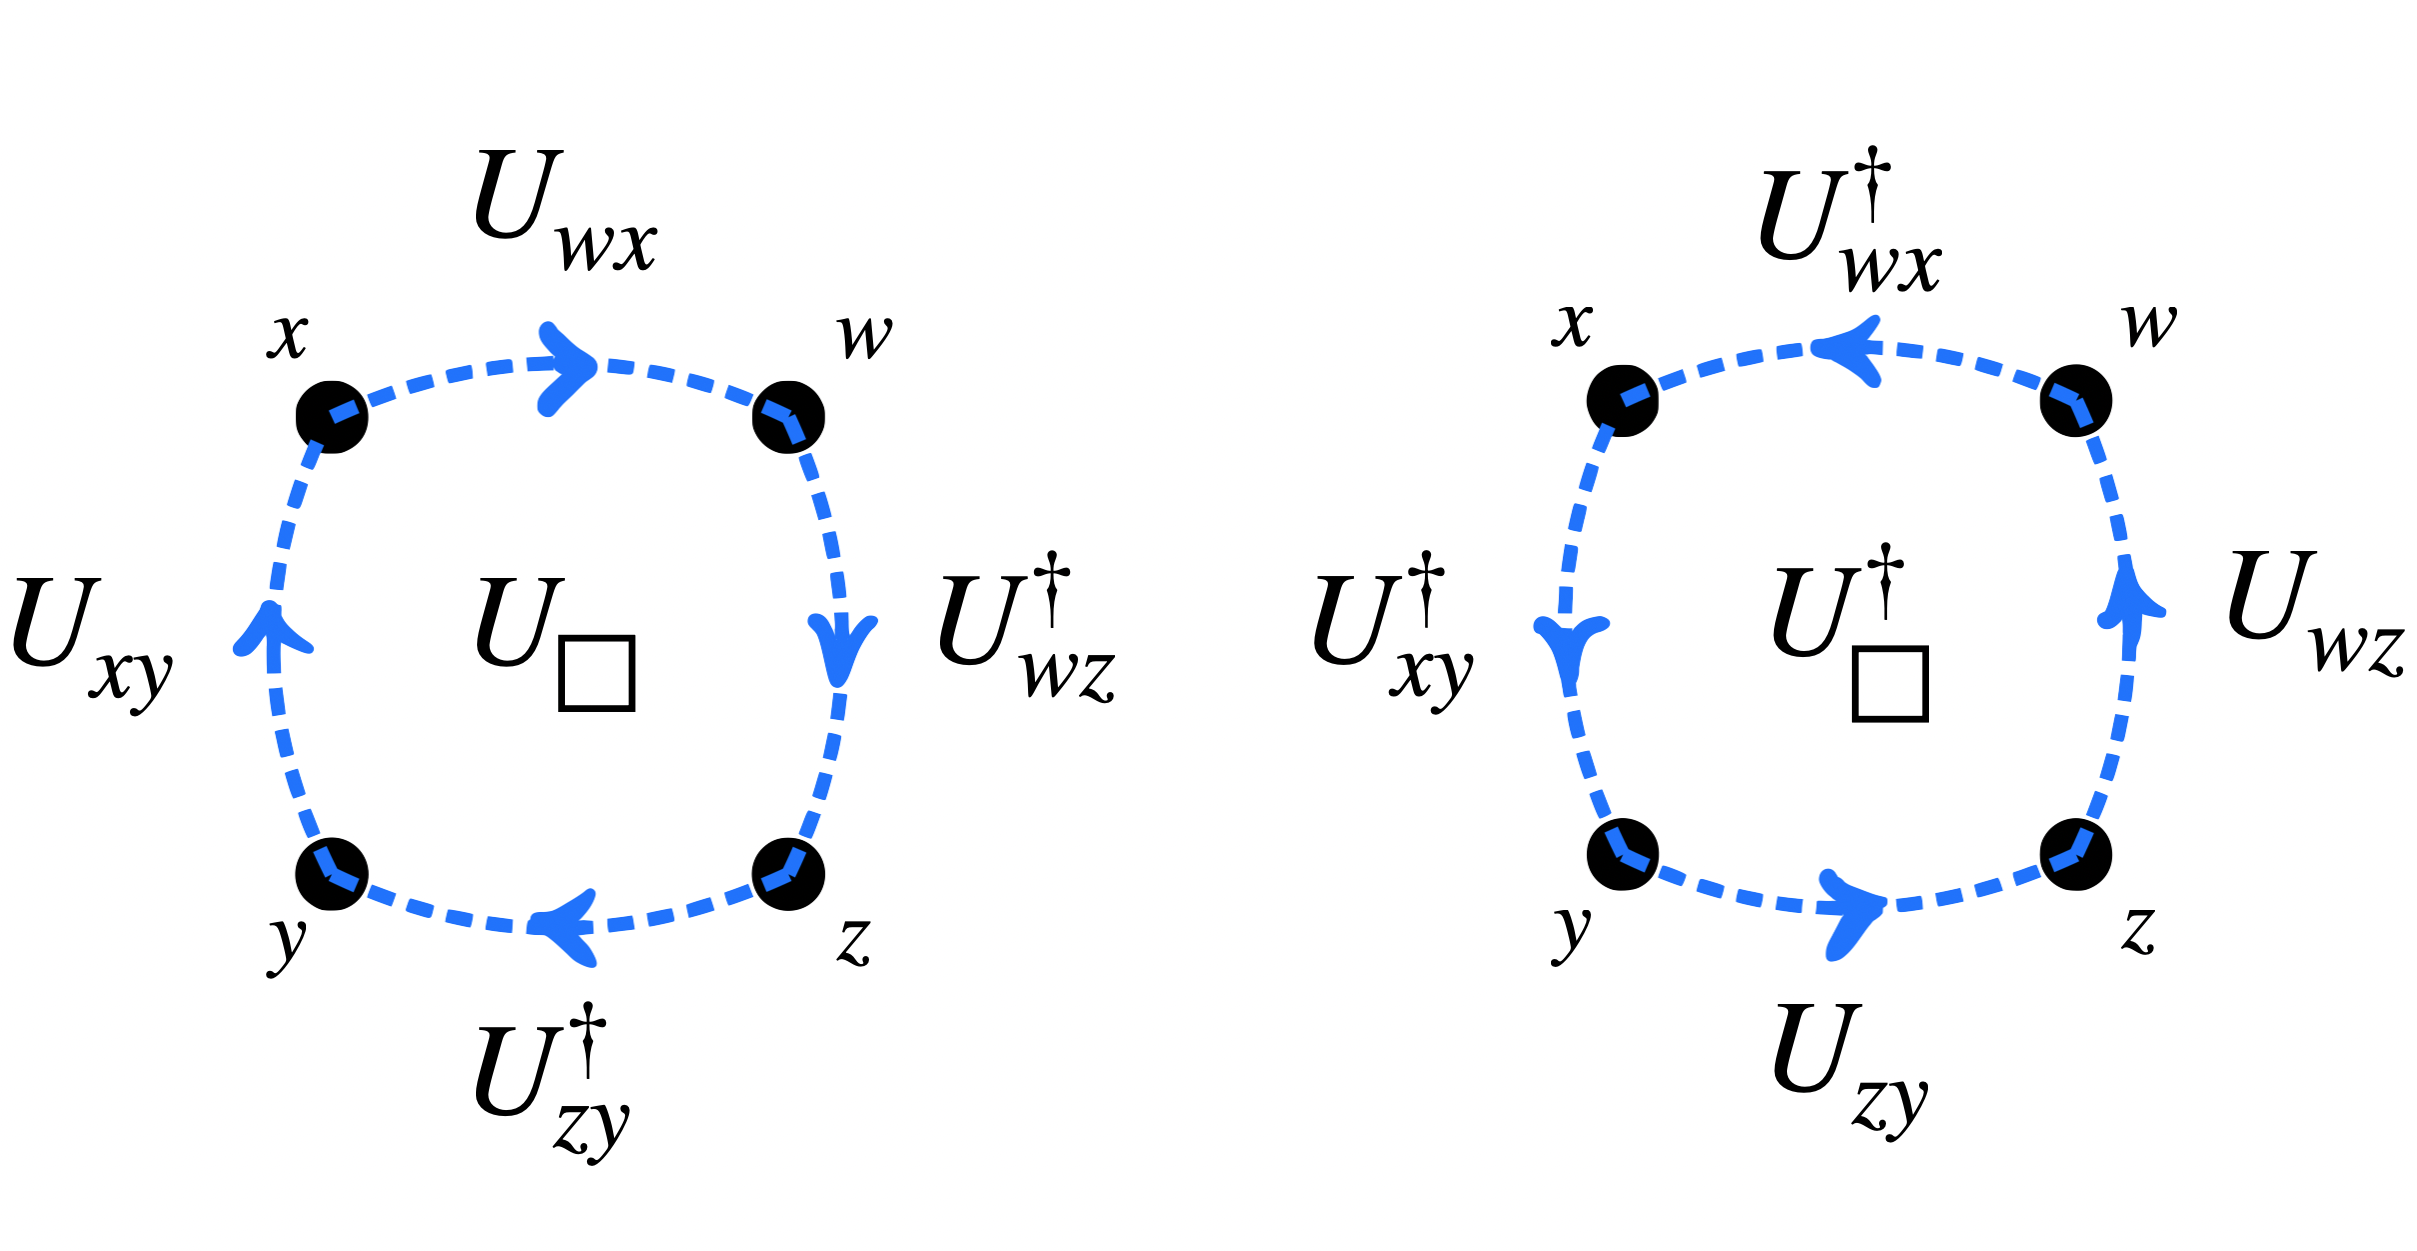
\includegraphics[width=\linewidth]{Usquare.png} % change jpg to pdf when doing the final compilation of the pdf
\end{subfigure}
\caption{Physical picture of the plaquette operators.\label{fig:Usq}}
\end{figure}

Then, by applying Stokes theorem in a single square loop in the lattice (view Figure \ref{fig:Usq} for reference),
\begin{equation}
    \iint_S \dd \vec{S} \cdot \vec{B} = \iint_S \dd \vec{S} \cdot ( \nabla \cross \vec{A}) = \oint_{\partial S} \dd \vec{r} \cdot \vec{A} = \oint_{wxyz} \dd \vec{r} \cdot \vec{A}(x),
\end{equation}
thus recovering the term in the exponent of $U^\dagger_\square$ (up to a change of sign). Using this relation between the plaquette terms and the magnetic field, the complete Hamiltonian in the lattice is written as \cite{wiese2013ultracold}
\begin{equation}
    H = -t \sum_{\expval{xy}}s_{xy}\left( \psi^\dagger_x U_{xy} \psi_y + \psi^\dagger_y U^\dagger_{xy} \psi_x \right) + m \sum_x s_x \psi^\dagger_x \psi_x + \frac{e^2}{2} \sum_{\expval{xy}} E^2_{xy} - \frac{1}{4e^2} \sum_\square \left( U_\square + U^\dagger_\square \right), \label{eq:HamQED}
\end{equation}
which is a Hamiltonian that for ($a \xrightarrow[]{} 0$) recovers QED. 

% . T
% \begin{equation}
%     \implies - \left( U_\square + U_\square^\dagger \right) = -2 \cos\left(e \oint_{\partial\square} \dd \vec{r} \cdot \vec{A} \right) \approx -2 + \left(e \iint_\square \dd \vec{S} \cdot \vec{B} \right)^2.% \sim (e {B}_\square)^2.
% \end{equation} 
% So the sum of plaquettes $U_\square$ is connected to the norm square of the magnetic field in each lattice loop, such that we can write the complete discrete Hamiltonian in the lattice as
In summary, we have discussed the connection between the transporter (gauge field) and electromagnetic fields in the lattice. In particular, with the transporter, the gauge field can be discretized, and it gives the physical interpretation of the $A_k(x)$ gauge field living on the lattice links and mediating the fermion-fermion interaction from neighboring sites.
% Notice that this interaction in the lattice is analogous to the interactions present in QED.


\subsection{Physical interpretation and symmetry remarks}

% \subsubsection{Gauss' law}
One important property of gauge symmetry is that the symmetry group has generators, which due to gauge symmetry, commute with the Hamiltonian operator. For the lattice QED on Wilson's formulation, the generator $G_x$ can be defined as:
\begin{equation} \label{eq:Gx}
    G_x = \psi^\dagger_x \psi_x + \sum_k \left( E_{x,x+\hat{k}} - E_{x-\hat{k},x}  \right), \quad \left[ H,G_x \right] = 0.
\end{equation}

Furthermore, the operator resembles closely what a discrete Gauss' law would be because we have a term similar to a charge density at the lattice site, and a divergence of the electric field around a lattice site.
% This interpretation intuitively tells us that Gauss' law is also valid in the discrete lattice, which is a desirable property to justify its physical relevance, as it reproduces expected dynamics when taking the lattice to the continuum.

For completeness, we can use the generator to define a general gauge transformation as an operator $V$
\begin{equation}
    V = \prod_x \exp(i e \alpha_x G_x),
\end{equation}
where $\alpha_x$ are the weights to the gauge transformation at each lattice site, analogous to a general gauge transformation in the continuous gauge theory.

The transformations in the local elements of the Hamiltonian are thus
\begin{equation}
    V\psi_x V^\dagger = \Omega_x \psi_x, \quad V \psi^\dagger_x V^\dagger = \psi^\dagger_x \Omega^\dagger_{x}, \quad V U_{xy} V^\dagger = \Omega_{x} U_{xy} \Omega^\dagger_{y},
\end{equation}
where $\Omega_z = \exp(ie\alpha_x)$. Substituting these transformations into the Hamiltonian in (\ref{eq:HamQED}) proves its gauge invariance.



% \begin{itemize}
%     % \item Discuss role of $\Phi$ here maybe ommit it
%     \item Discuss interpretation of Gauss' law
%     \item Discuss the generators of symmetry in terms of a local discrete Gauss law
%     \item How Gauge symmetry appears
% \end{itemize}
% \subsection{Concluding remarks}

Wilson's formulation was introduced, and it allows defining lattice gauge theories. However, even in this lattice formulation, the Hilbert space of each lattice link is unbounded. This becomes a problem if we try to perform simulations of this quantum system with quantum resources with bounded Hilbert spaces (e.g. qubits).
% To alleviate this problem, the quantum link model is introduced in the next section.

% , which can somewhat alleviate this problem while also generalizing how a lattice model can be defined.
% ow these problems might be alleviated with some useful simplifications.


% to define Hamiltonians in discrete lattices. We can argue that these lattices present very useful symmetric properties that when taking them to the continuous limit, one would expect to recover the physical behavior of continuous field theories (up to certain considerations and when taking care of problems like the fermion doubling). 


% 











% \subsection{Fermion doubling}
% % \textit{(Still needs transcribing from paper to this document)}
% % \subsubsection{Seen within the lattice}
% Consider the naive approach in which we define a discrete fermionic field in a square lattice of (2+1) dimensions (2 for discrete space, 1 for a continuous-time). We can describe the interactions of 2 nearest neighbors fermions (n.n.) via the Action of the Free Dirac fermion

% \begin{equation} \label{eq:DiracFreeAction}
%     \mathcal{S} = \int \dd^d x \overline{\psi}(i \cancel\partial - m) \psi
% \end{equation}

% And to perform a discretization of this action, we can propose the following action:
% \begin{align}
%     S &= a^d \sum_{x,\mu} \left[ \overline{\psi}_x \frac{i\gamma^\mu}{2a}  \psi_{x+\mu} - \overline{\psi}_{x+\mu} \frac{i\gamma^\mu}{2a} \psi_x \right] - a^d \sum_x \overline{\psi}_x\psi_x\\
%     S &= a^d\, \overline{\psi}_x D_{x,y} \psi_y \quad \textnormal{for} \quad D_{x,y} = \sum_\mu \frac{1}{2a}(\gamma_\mu \delta_{x+\mu,y} - \gamma_\mu \delta_{x-\mu,y}) - m\delta_{x,y} 
% \end{align}
% Where $a$ is the lattice parameter, and $\mu$ counts over the nearest neighbours' directions. More importantly, $\psi$ represents a discretization of the fermion field.

% Note that in the $a\xrightarrow[]{}0$ (continuous limit), reproduces (\ref{eq:DiracFreeAction})

% However, it does not reproduce the expected physical behavior. To observe this, and without going much into detail, we can compute the following expectation value in this discrete lattice, in momentum space.

% \begin{equation}
%     \expval{\overline{\psi}(-p)\psi(p)} = \left[ i \sum_\mu \gamma_\mu \frac{1}{a} \sin (p^\mu a) + m\right]^{-1}
% \end{equation}

% This result gives us 2 poles in the expectation value: at $p^\mu$ and at $p^\mu = \pi/a$ for each of the directions $\mu$. Thus, doubling our fermion count as $2^d$, where $d$ is the number of spatial directions in our lattice. 

% We thus need to propose a different discretization procedure for our lattice, or on the other hand, re-interpret our extra fermions as extra degrees of freedom of the fermionic field (flavors, etc.)








\section{Quantum link models}

Quantum link models are a generalization of the previous formulation that allows defining Hamiltonians whose operators have bounded Hilbert spaces. In basic terms, they are made of sites and links, whose properties and interactions are mediated by a Hamiltonian. Notice that the quantum link models still recover gauge invariance in the lattice and they can be sent to their continuous limit \cite{wiese2013ultracold}.

% Quantum link models that effectively recover Abelian (like QED) and Non-Abelian (like QCD) gauge theories (even though in the discrete lattice they only present discrete symmetries).



\subsection{U(1) quantum link model in (2+1) dimensions}

To define a lattice with U(1) quantum link model, we can define the electric field $E_{xy}$ and the transporter $U_{xy}$ as spin$-1/2$ operators in the following way:
\begin{align}
    U_{xy} &\mapsto S_{ij}^1 + iS_{ij}^2 = S_{ij}^{+},\\
    U^\dagger_{xy} &\mapsto S_{ij}^1 - iS_{ij}^2 = S_{ij}^{-},\\
    E_{xy} &\mapsto S_{ij}^3,
\end{align}
where $i$ and $j$ refer to the lattice sites that are linked. The spin commutation relations $\left[ S_{jk}^a,S_{j'k'}^b \right] = i \delta_{jj'}\delta_{kk'}\epsilon^{abc}S^c_{jk}$ imply that in the quantum link model, we recover (\ref{eq:comEU}) and (\ref{eq:comEUt}). Although we do not recover the analogous of (\ref{eq:comUU}):
\begin{equation}
    \left[ S^{+}_{jk}, S^{-}_{j'k'}\right] = 2 \delta_{jj'}\delta_{kk'}S^3_{jk}.
\end{equation}

The fermionic fields $\psi_{x}$ are rewritten as fermionic annihilation and creation operators at each site (they are the same object but now called $c_i$ and indexed by $i$)
\begin{align}
    \psi_x &\equiv c_i \\
    \psi_x^\dagger &\equiv c^\dagger_i.
\end{align}
The Hamiltonian terms from (\ref{eq:HamQED}) are rewritten respectively as
% \begin{equation}
%     H_t = -t \sum_{\expval{ij}} \left[ c^\dagger_i S^+_{ij} c_j + \textnormal{h.c.} \right],
% \end{equation}
% \begin{equation}
%     H_m = m \sum_i (-1)^i c^\dagger_i c_i,
% \end{equation}
% For the gauge field, the last two terms in (\ref{eq:HamQED}) turn into
\begin{align}
    H_t &= -t \sum_{\expval{ij}} \left[ c^\dagger_i S^+_{ij} c_j + \textnormal{h.c.} \right],\\
    H_m &= m \sum_i (-1)^i c^\dagger_i c_i,\\
    H_E &= \kappa \sum_{\expval{ij}} (S^3_{ij})^2,\\
    H_\square &= -J \sum_\square \left[ S^+_{li} S^+_{ij} S^-_{kj} S^-_{lk} + \textnormal{h.c.}\right],
\end{align}
such that the QED quantum link model in the $(2+1)$ dimensional lattice has the following Hamiltonian:
\begin{equation}\label{eq:HamLQED}
    H = H_t + H_m + H_E + H_\square. %+ H_V.
\end{equation}

% There is also an extra term now that refers to the flipping of whole plaquettes in the lattice with a certain potential
% \begin{equation}
%     H_V = V \sum_\square \prod_{(ij) \in \square} S^3_{ij}.
% \end{equation}
% In total, the complete

\subsubsection{Remarks about the U(1) quantum link model's Hilbert space}

Given that our Hamiltonian from (\ref{eq:HamLQED}) is now in the context of a quantum system, we can discuss further which states are physically allowed. In essence, the physical Hilbert space is the gauge-invariant Hilbert space, defined as
\begin{equation}
    \mathcal{H}_G = \left\{ \ket{\psi}\, \text{s.t.}\, G_i\ket{\psi} = 0 \quad \forall\, i \right\},
\end{equation}
where $\ket{\psi}$ corresponds to the quantum state consisting of all fermions and spins in the lattice sites and links respectively. $G_i$ can be defined from (\ref{eq:Gx}). Recall that a physical interpretation of the generators of a gauge symmetry is that they are Gauss' laws, so our physical Hilbert space corresponds to all quantum many-body wave functions that comply with these laws. Moreover, given that the gauge symmetry for QED ($U(1)$ gauge theory) has only 1 generator, there is only 1 Gauss' law that separates the physical from the nonphysical quantum states.

% ??? ADD EXAMPLE ON INVARIANCE OF QUANTUM STATES
% The lattice QED Hamiltonian in a (2+1) dimension system can then be written as
% \begin{equation}
%     H_{QED} = -J\sum_x
% \end{equation}

To illustrate this, consider the ground state of a quantum link model consisting of a chain. The ground state would consist of fermions in the anti-particle sites (yellow sites), and no fermions in the particle sites (blue sites). The number inside the sites are occupations on the number basis. The links are all in the same spin state (due to Gauss' law). The numbers below the sites are the site label ($i$). Then, the first energy excitation could be obtained by applying the hopping term as shown in Figure \ref{fig:gnd}.

\begin{figure}[h!]
\centering
\begin{subfigure}{0.4\textwidth}
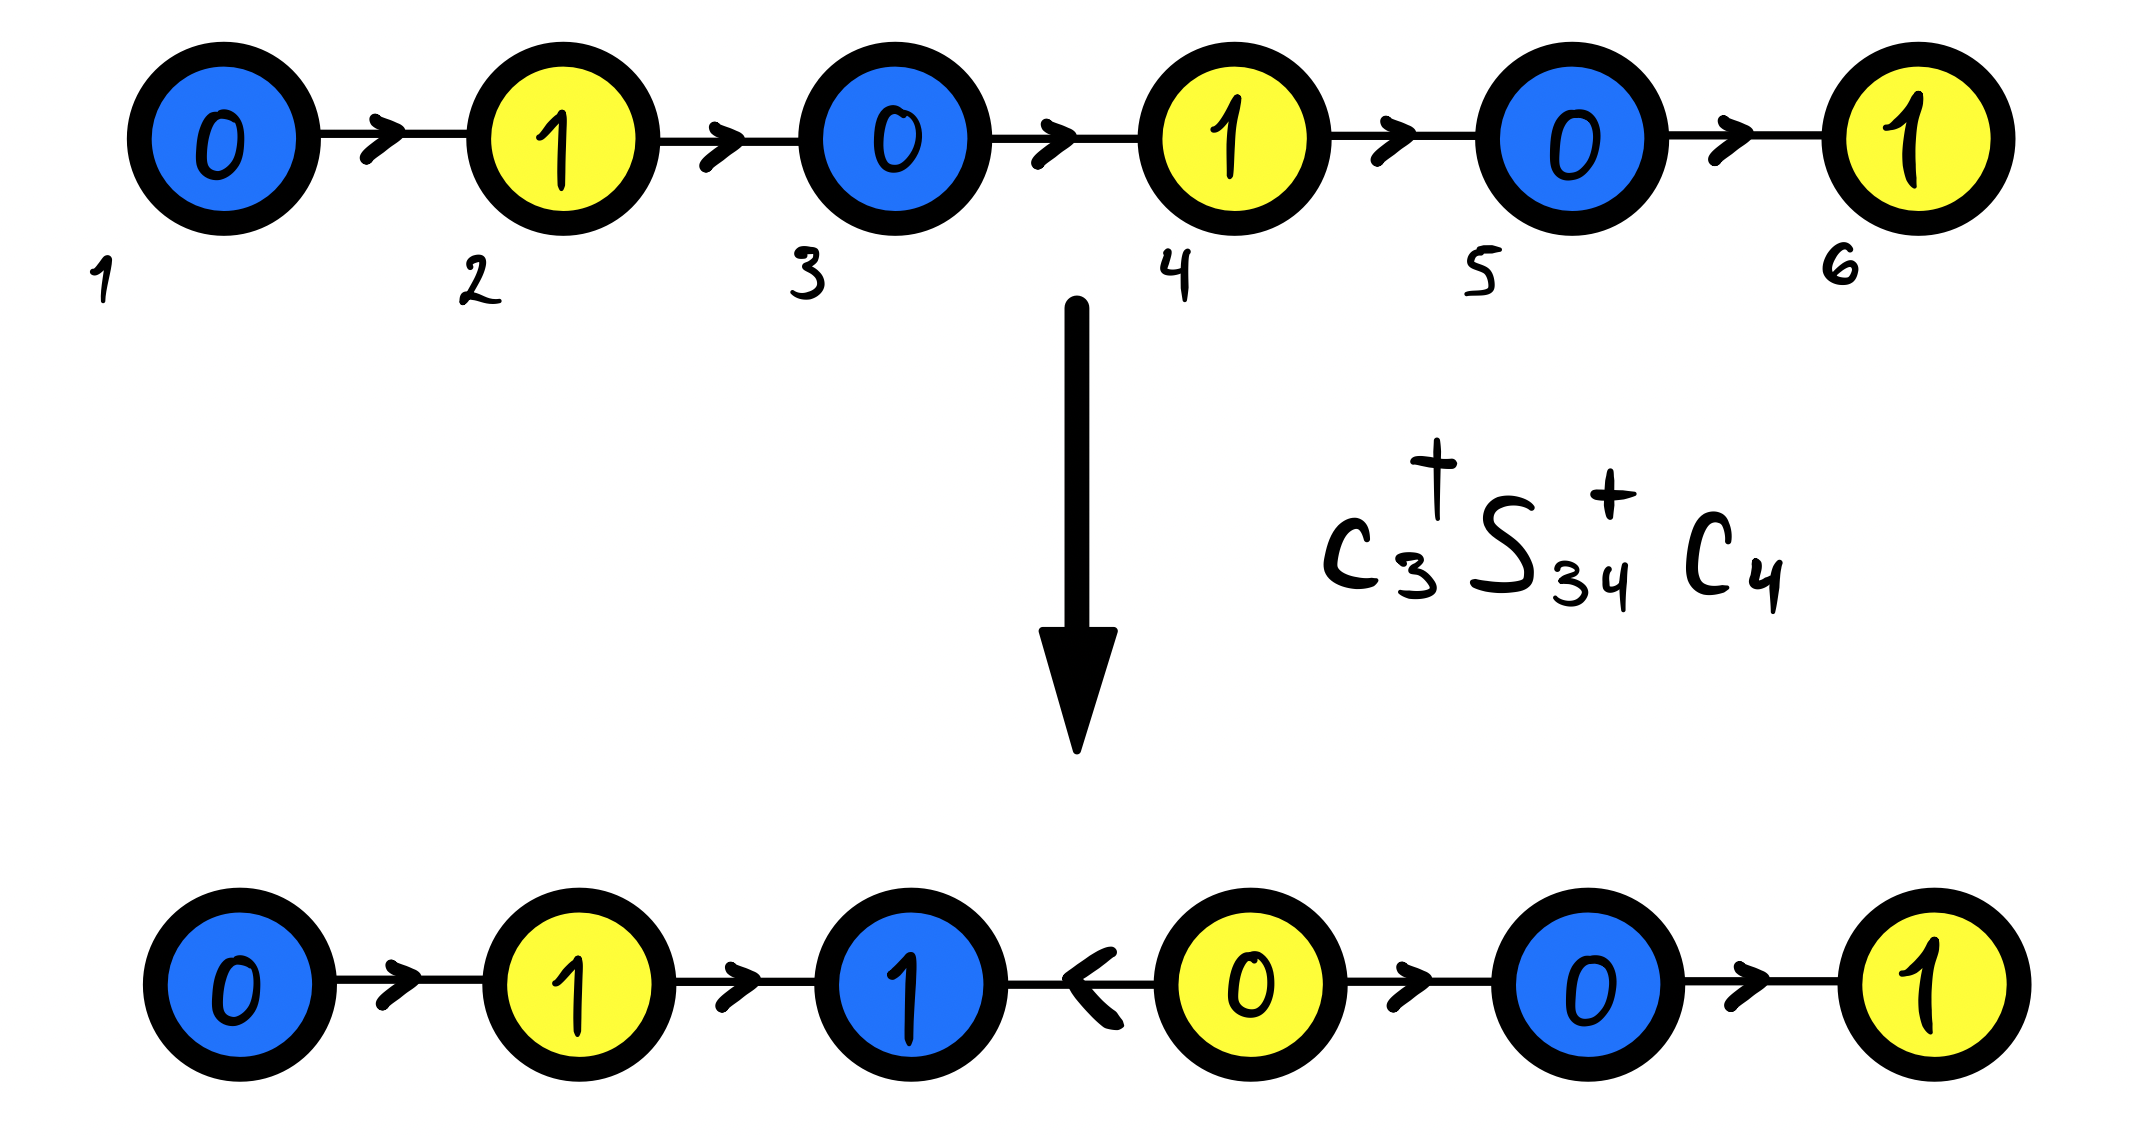
\includegraphics[width=\linewidth]{GndState.png} % change jpg to pdf when doing the final compilation of the pdf
\end{subfigure}
\caption{Application of a hopping term on the ground state.\label{fig:gnd}}
\end{figure}
The hopping term represents the creation of a particle-antiparticle pair, while the spin at the link flips to represent a change in the electric field. After the hopping, the Gauss' law is still valid.

\subsection{SU(N) quantum link model in (1+1) dimensions}

In this section, the definition of a quantum link model with non-Abelian gauge symmetry is presented. Although there are generalizations to higher spatial dimensions, here we consider the case of a chain (1+1)-dimensional system. Without much discussion about its derivation, the theory consists of a chain of sites in which each site holds a pair of fermionic \textit{rishon} operators with flavors ($m$) encoding the $SU(N)$ representation that we write the theory on.
\begin{equation}
    c^{\alpha,(m)}_{R;j} \qquad \textnormal{and} \qquad c^{\beta,(m)}_{L;j+1},
\end{equation}
where $\alpha$ and $\beta$ correspond to the color indices, and take values from $1$ to $N$. The gauge field is made up of the following operator:
\begin{equation}
    U^{\alpha \beta}_{j,j+1} = c^\alpha_{R;j} c^{\beta\dagger}_{L;j+1},
\end{equation}
and in the lattice sites, there are fermionic operators $\psi^\alpha_j$ corresponding to the matter fields.

The $N^2-1$ generators for the $SU(N)$ symmetry are
\begin{equation}
    G^\gamma_j = \psi^{\alpha \dagger}_j \lambda^\gamma_{\alpha \beta} \psi^\beta_j + L^\gamma_j + R^\gamma_j,
\end{equation}
for $\lambda^\gamma$ the SU(N) Gell-Mann matrices, and $L$, $R$ the non-Abelian flux operators (similar to the electric field terms in (\ref{eq:Gx}), they carry the flux of the bosons to the left and right lattice sites). 

The flux operators are defined as
\begin{align}
    L^\gamma_j = c^{\alpha \dagger}_{L;j} \lambda^\gamma_{\alpha \beta} c^\beta_{L;j},\\
    R^\gamma_j = c^{\alpha \dagger}_{R;j} \lambda^\gamma_{\alpha \beta} c^\beta_{R;j}.
\end{align}
Finally, the Hamiltonian for a $SU(N)$ quantum chain model is defined as \cite{dalmonte2016lattice}
\begin{multline}
    H_{SU(N)} =  -t \sum_j \left[ \left( \psi^{\alpha \dagger}_j c^\alpha_{R;j} \right)\left( c^{\beta \dagger}_{L;j+1} \psi^{\beta}_{j+1} \right) + \textnormal{h.c.} \right] + m \sum_j\left( -1 \right)^j\,\psi^{\alpha \dagger}_j \psi^\alpha_j\\
    + \frac{g^2}{2}\sum_j \left[ L^\alpha_j L^\alpha_j + R^\alpha_j R^\alpha_j \right] + \epsilon \sum_j \left( \prod_{\kappa=1}^N c^{\kappa \dagger}_{R;j} c^{\kappa}_{L;j+1} + \textnormal{h.c.} \right),
\end{multline}
where the respective terms can be interpreted as energy coming from the interaction (hopping) of fermions between neighboring sites, the energy from the fermionic matter, the energy from the gauge field flux, and the energy from the gauge bosons. 
% Importantly for quantum simulation, this Hamiltonian can be encoded into qubit sites.


\subsubsection{Remarks about the SU(N) quantum link model's Hilbert space}

Analogous to the case for the U(1) theory, the $N^2-1$ generators in this theory are symmetries of the Hamiltonian such that $\left[ G^\gamma_j, H \right] = 0$ for $\gamma = \{1,2,\dots N^2-1\}$. Each generator implies an independent Gauss' law, which restricts the physical Hilbert space to the space of quantum states that comply with
\begin{equation}
    G^\gamma_j \ket{\psi} = 0, \quad \forall \,j \,\, \forall \gamma.% = \{1,2,\dots,N^2-1\}.
\end{equation}
% For the relevant case of $SU(3)$ gauge symmetry, the continuous analogous to the quantum link model is QCD, where the 8 generators correspond to 8 gluons, and the Gauss' laws are related to the conservation of color charge.
%  that there are generalizations into higher dimensional systems (https://arxiv.org/pdf/hep-lat/0110148.pdf).% CHANGE WORDING

% DELETE SU(N)

% \begin{itemize}
%     \item Discuss Hamiltonian in terms of Spin 1/2 operators
%     \item Compare commutation relationships and discuss the difference from continous symmetry to a discrete one
%     \item Argue relevance of QLM for Quantum Simulations
% \end{itemize}


% \textit{(We will discuss the staggered lattice case)}

% \subsection{Definitions to the fermionic variables on the lattice sites}

% \subsection{Defining the Hamiltonian}

% \subsection{Discussion on the Gauge group for this particular system setup}

% \section{"The general case"}

\section{Quantum simulations}

% \subsection{The struggles of classical computing for lattice gauge theories simulations}

To justify using quantum simulation algorithms in quantum computers instead of computational methods in classical computers, it is worth mentioning that classical computers may find it difficult to represent a quantum Hilbert space and perform estimates on it\footnote{However, there are classical computations that would be very hard to outperform with a quantum computer.}. Two relevant problems related to this are the following:

\subsubsection{Exponentially large Hilbert space}
The exponentially growing Hilbert space with system size $n$ needs an exponential amount of classical computer memory to represent a quantum state. Consider for instance having a cubic lattice of $n = 5 \times 5 \times 5 = 125$ sites. It will also have $3 n$ lattice links (periodic boundary conditions). At each lattice site and link, there is a qubit and for each qubit, we use 2 single-precision numbers to represent its wavefunction (2 angles in Bloch's sphere). This means that the total amount of memory (1 float = 4 bytes) needed to represent one wavefunction in this lattice is $4\cdot2^{4n} \text{bytes} \approx 10^{151} \text{bytes}$.

\subsubsection{Sign problem}
One way of alleviating this problem in classical computation is by using Monte Carlo methods that sample accurately the system's Hilbert space. In this case, expectation values can be performed as
\begin{equation}
    \expval{O}_p = \frac{\sum_{\{\ket{\psi}\}} \ev{O}{\psi} p_{\ket{\psi}} }{\sum_{\{\ket{\psi}\}} \braket{\psi} p_{\ket{\psi}} },
\end{equation}
where as the notation suggests, the expectation value depends on the sampling function $p$. A choice for the sampling function is
\begin{equation}
    p_{\ket{\psi}} = \exp{- {S}({\ket{\psi}})}.% or with the action 
\end{equation}
Then the sign problem appears whenever $p_{\ket{\psi}}$ becomes negative (or, not a positive real number) \cite{chandrasekharan1999meron}.


%, which aims at accurately estimating expectation values in an exponentially large Hilbert space with random sampling the other problem is ofter referred to as the sign problem, it occurs when which is due to the very large oscillations found in the action of the system (note that some computational methods are based on randomly sampling quantum states and computing its probability via how to perform estimates of expectation values of these systems. In essence, these two main problems are the exponentially growing size of the lattice's Hilbert space and the sign problem. 

These problems do not become relevant in the quantum simulations realm, because quantum computing inherent can access a Hilbert space exponential with the system size $n$, and performing expectation values correspond to doing measurements at the end of a quantum algorithm (not susceptible to the sign problem). 
% As a side note, arguably the most natural way to simulate a quantum system is through a quantum computer.
%  expectation value not done by hand, but from the quantum state.

\subsection{Transformations for different quantum platforms}

To adapt our Hamiltonian between different operator statistics, we can make use of two transformations: the Holstein-Primakoff transformation to approximate spin operators via bosonic operators, and the Jordan-Wigner approximation to transform between spin and fermionic operators.

\subsubsection{Holstein-Primakoff transformation}

This is a transformation that considers we can reproduce expectation values of bosonic wavefunctions with $N = 2s+1$ spin$-s$ states, by truncating the bosonic Hilbert space to the first $N$ bosonic functions ($\{ \ket{0},\ket{1},\dots,\ket{N-1}$ in the number basis). The transformation requires us to establish an equivalence between the vacuum state $\ket{0}_B$ and the state $\ket{s,m_s=+s}$ of a spin$-s$ particle, and then the action of the creation operators acts analogous to lowering the spin $z$ projection number:
\begin{equation}
    \ket{s,s-n} \mapsto \frac{1}{\sqrt{n!}}\left( a^\dagger \right)^n \, \ket{0}_B.
\end{equation}
Then, the operators are equivalent in the following way:
\begin{align}
    S^+ = S^1 + iS^2 &= \sqrt{2s} \, \sqrt{1-\frac{a^\dagger a}{2s}} \, a, \\
    S^- = S^1 - iS^2 &= \sqrt{2s} \, a^\dagger \, \sqrt{1-\frac{a^\dagger a}{2s}}, \\
    S^3 &= (s-a^\dagger a).
\end{align}
Thus, in principle we can transform the spin terms into a bosonic representation and perform a quantum simulation in a bosonic lattice (e.g. cold atoms).

Notice that fundamentally, both operators are different because bosonic creation/annihilation operators span an infinite dimensional Hilbert space (Fock space), while each spin$-s$ operator spans only a finite dimensional Hilbert space of size $2s+1$. Nevertheless, the bosonic commutation relations imply:
\begin{align}
    \left[ S^+,S^- \right] &= 2S^3,\\
    \left[ a,a^\dagger \right] &= 1,\\
    \left[ a,a \right] = \left[ S^+, S^+ \right] &= 0,
\end{align}
which are the expected commutation relations for spin operators. More details can be found in the appendices to this report.

\subsubsection{Jordan–Wigner transformation}

The Jordan-Wigner transformation allows us to change from spin$-s$ operators to fermionic creation and annihilation operators and viceversa. For a spin lattice, where all the sites are indexed by a single number $i$ (only 1 index even in higher dimensional lattices), to properly recover the fermionic anti-commutation relations
\begin{align}
    \{a_i,a^\dagger_j\} &= \delta_{ij},\\
    \{a_i,a_j\} &= 0,\\
    \{a^\dagger_i,a^\dagger_j\} &= 0,
\end{align}
we can make the following definition via spin$-1/2$ operators:
\begin{align}
    a^\dagger_j &= \exp[+i\pi \sum_{k=1}^{j-1} S_k^+S_k^-] \, S_j^+,\\
    a_j &= \exp[-i\pi \sum_{k=1}^{j-1} S_k^+S_k^-] \, S_j^-,\\
    a^\dagger_j a_j &= S_j^+ S_j^-.
\end{align}
Inversely, we can write spin operators via fermionic operators:
\begin{align}
    S_j^+ &= \exp[-i\pi \sum_{k=1}^{j-1} a_k^\dagger a_k] \, a_j^\dagger,\\
    S_j^- &= \exp[+i\pi \sum_{k=1}^{j-1} a_k^\dagger a_k] \, a_j,\\
    S_j^3 &= 2a_j^\dagger a_j - 1.
\end{align}
% Notice that the transformation is non-local.
% For a system of higher spatial dimension, the transformation is applied by labeling all sites with 1 single index. 

% To justify the advantages of simulating a quantum system with the use of quantum computers are varied but ultimately rely on the ability of a quantum computer to encode quantum states and dynamics in a much more efficient and natural way. So to complete this report's discussion, our last step is to discuss the different methods that can be employed to dissect the Hamiltonian and transform its time evolution into an algorithm.



% qubits, we require wanting a lower error bound implies needing a larger complexity both in how many qubits we operate, and how many gates are required for a time-step.


\subsection{Digital quantum simulation}
% \subsubsection{Hamiltonian in time-steps}

Given that now we can define a lattice Hamiltonian in terms of convenient operators for our quantum computing platform, we shall discuss how we proceed and split up the Hamiltonian evolution of our system. Although the simulations that can be done experimentally still need much progress in error control and the number of qubits that can be used, algorithms are already developed to perform digital quantum simulations. These algorithms in principle allow for a large-scale simulation of a lattice gauge theory with a quantum computer.

% To simulate Hamiltonian dynamics in a quantum system, there are algorithms that in principle perform an approximated time evolution of a quantum system. 
The algorithms are based on decomposing the Hamiltonian operator and evolving in discrete time steps. The decomposition can be done by product formulas, discrete-time quantum walks, linear decomposition of unitaries, etc. \cite{childs2018toward} The performance that we can expect in a quantum simulation depends on the specific algorithm used and the number of qubits in the simulation. As a general rule, to achieve a lower error bound or to simulate a larger system, we require more gates. An advantage that digital quantum simulations offer is that it is possible to obtain theoretical asymptotic bounds to the gate complexity (amount of gates) required to achieve a given error $\epsilon$ or a given amount of qubits $n$ \cite{childs2018toward}.

\subsubsection{Product formula algorithm}

The product formula is a way to approximate the exponential of a sum of operators. Although this might be trivial for an exponential of a sum of numbers, this decomposition becomes complicated for non-commuting operators. Nevertheless, the terms coming from the commutation of the operators can be made to be small in a limit. To motivate the approximation, let us look at Zassenhaus' result:
\begin{equation}
    e^{t(X+Y)} = e^{tX}\,e^{tY}\,e^{-t^2 \left[X,Y\right] /2} \,e^{t^3(2\left[Y,\left[X,Y\right]\right] + \left[X,\left[X,Y\right]\right])/6} \, \dots . 
\end{equation}
Naively, we can thus write down the first order approximation as
\begin{equation}
\exp\left(-it\sum_{j=1}^{L}\alpha_j H_j \right) \approx  \left[\prod_{j=1}^{L}\exp\left(-\frac{it}{r} \alpha_j H_j\right)\right]^r.
\end{equation}
The asymptotic error at this order can be found to be
\begin{equation}
    \norm{\exp\left(-it\sum_{j=1}^{L}\alpha_j H_j \right) - \left[\prod_{j=1}^{L}\exp\left(-\frac{it}{r} \alpha_j H_j\right)\right]^r } = \mathcal{O}\left(\frac{L\,t\,\alpha_{\text{max}}}{ \sqrt{r}} \right)^2,
\end{equation}
where $\alpha_{\text{max}} = \max_j \alpha_j$. To higher order, the approximation is the $(2k)^{\text{th}}$-order Suzuki formula, which gets a polynomial suppression in the error for each subsequent higher order.

% Derived from this formula, we can state the Suzuki-Trotter decomposition (unrelated to this work, but this decomposition is commonly used in one of the derivations of the Path Integral for quantum mechanics)
% \begin{equation}
%     e^{X+Y} = \lim_{N\xrightarrow[]{}\infty} \left( e^{X/N} \,e^{Y/N}  \right)^N,
% \end{equation}
% where $X,Y$ are arbitrary $\mathbb{C}_{n\times n}$ matrices.

% To higher order, the approximaiton is the $(2k)^{\text{th}}$-order Suzuki formula:
% \begin{align}
%     S_2 (\lambda) &= \prod_{j=1}^L e^{\alpha_j H_j \lambda/2} \prod_{j=L}^1 e^{\alpha_j H_j \lambda/2},\\
%     S_{2k}(\lambda) &= \left[S_{2k-2}(p_k\lambda)\right]^2\, S_{2k-2}\left(\lambda(1-4 p_k)\right)\,\left[S_{2k-2}(p_k\lambda)\right]^2,\\
%     \implies &\exp\left(-it\sum_{j=1}^{L}\alpha_j H_j \right) \approx  \left[S_{2k}\left(-\frac{it}{r}\right)\right]^r,
% \end{align}
% where $p_k = 1/\left(4-4^{1/(2k-1)}\right)$, $k>1$. Once again, the asymptotic error can be obtained and in particular, it gets a polynomial suppression for each subsequent higher order.
% \begin{equation}
%     \norm{\exp\left(-it\sum_{j=1}^{L}\alpha_j H_j \right) - \left[S_{2k}\left(-\frac{it}{r}\right)\right]^r } = \mathcal{O}\left(\frac{(L\,t\,\alpha_{\text{max}})^{2k+1}}{ r^{2k}} \right).
% \end{equation}
In fact, it is possible to derive upper bounds for the error. For the 1$^{\text{st}}$ order:
\begin{align}
    \norm{\exp(-it \sum_{j=1}^L H_j) - \left[ \prod_{j=1}^L \exp(-\frac{it}{r} H_j) \right]^r } \leq \frac{(L\Lambda t)^2}{r}\exp(\frac{L\Lambda \abs{t}}{r}),
\end{align}
where $\Lambda = \max_j \norm{H_j}$. Therefore, we can define the minimum $r$ values to achieve the desired maximum norm error $\epsilon$
\begin{align}
    r_1 &= \left\lceil \max \left\{ L \Lambda \abs{t},\, \frac{e(L\Lambda t)^2}{\epsilon} \right\} \right\rceil.\\
    % r_{2k} &= \left\lceil \max \left\{ 2L5^{k-1}\, \Lambda \abs{t},\, \sqrt[2k]{ \frac{e(2L5^{k-1}\, \Lambda \abs{t})^{2k+1}}{3\epsilon} }  \right\} \right\rceil.
\end{align}

% For the $(2k)^\text{th}$ order formula, the error is further bounded
% \begin{equation}
%     \norm{\exp(-it \sum_{j=1}^L H_j) - \left[ S_{2k}\left(-\frac{it}{r} \right) \right]^r } \leq \frac{(2L5^{k-1}\,\Lambda \abs{t})^{2k+1}}{3r^{2k}}\exp(\frac{2L5^{k-1}\,\Lambda \abs{t}}{r}).
% \end{equation}
% \subsection{More advanced algorithm}

While the Product formula algorithm might seem simple to understand conceptually, other algorithms make use of more powerful quantum resources, like ancillary states, to reduce the complexity of the final routine, while also being able to keep a desired bound on the error \cite{childs2018toward}.

% TABLE


\section{Concluding remarks}

Some gauge theories are useful for modeling the fundamental processes in nature. As discussed in this report, there is a procedure that allows discretizing them into lattice gauge theories: Wilson’s formulation. This formulation involves quantum operators with unbounded Hilbert spaces, so quantum link models were introduced, which can be made up of only quantum operators with bounded Hilbert spaces, and thus are convenient for simulation purposes.

A discussion on how to model lattice gauge theories using these quantum link models was presented for a $U(1)$ gauge theory and a $SU(N)$ gauge theory. Furthermore, the Holstein-Primakoff and the Jordan-Wigner transformations were introduced, which allow relating bosonic or fermionic operators to spin operators. In principle, a quantum link model can thus be made with a lattice of spins.

Finally, a short review of the product-formula algorithm was presented, which allows in principle to study lattice gauge theories via quantum link models.




\section{Acknowledgments}
I would like to acknowledge the helpful guidance by Dr. Joao Pinto Barros in the realization of this report, and in the planning for the proseminar talk given on March 28, 2022.



% Another possible algorithm we can use in order to simulate our Hamiltonian is to implement a truncated expansion of the time evolution operator ($\exp(-itH)$). We can define the truncated sum as
% \begin{equation}\label{eq:tildeU}
%     \tilde{U} = \sum_{k=0}^K \frac{(-itH)^k}{k!},
% \end{equation}
% where we can see that we recover the exact time evolution by taking the limit $K\xrightarrow[]{}\infty$.

% Now, given that we can express our Hamiltonian as
% \begin{equation}
%     H = \sum_{l=1}^L \alpha_l H_l,
% \end{equation}
% our expression in (\ref{eq:tildeU}) can be rewritten in terms of a sum of unitaries $V$:
% \begin{align}
%     \tilde{U} &= \sum_{k=0}^K \sum_{l_1,\dots,l_k = 1}^L \, \frac{t^k}{k!}\,\alpha_{l_1}\dots\alpha_{l_k} \,(-i)^k H_{l_1}\dots H_{l_k} \label{eq:UalphasHs}\\ 
%      &= \sum_{\gamma=0}^{\Gamma-1}  \, \beta_\gamma \tilde{V}_\gamma,
% \end{align}
% where $\Gamma = \sum_{k=0}^K L^k$.



\newpage
\addcontentsline{toc}{section}{Bibliography}

\bibliographystyle{unsrt}
\bibliography{refs}



\newpage

\begin{appendices}

\section{Holstein-Primakoff transformation commutation relations}

To observe directly the relationship between the commutation relationships of spin operators and bosonic operators, let us prove that we recover the spin commutation relations from bosonic commutation relations when we apply the Holstein-Primakoff transformation.

The transformation is defined as
\begin{align}
    S^+ = S^1 + iS^2 &= \sqrt{2s} \, \sqrt{1-\frac{a^\dagger a}{2s}} \, a, \label{eq:ASp}\\
    S^- = S^1 - iS^2 &= \sqrt{2s} \, a^\dagger \, \sqrt{1-\frac{a^\dagger a}{2s}}, \label{eq:ASm}\\
    S^3 &= (s-a^\dagger a) \label{eq:AS3}.
\end{align}
Moreover, the bosonic creation and annihilation operators have the following commutation relations
\begin{align}
    \left[ a , a^\dagger \right] &= 1, \\
    \left[ a , a \right] &= 0, \\
    \left[ a^\dagger , a^\dagger \right] &= 0.
\end{align}
Now, let us compute the commutation relationship of the operators defined in (\ref{eq:ASp}), (\ref{eq:ASm}), (\ref{eq:AS3}):
\begin{align*}
    \left[ S^+,S^- \right] &= S^+ S^- - S^- S^+, \\
    &= 2s \left( \sqrt{1-\frac{a^\dagger a}{2s}} a a^\dagger \sqrt{1-\frac{a^\dagger a}{2s}} - a^\dagger \sqrt{1-\frac{a^\dagger a}{2s}} \sqrt{1-\frac{a^\dagger a}{2s}} a \right),\\
    &\text{taking $a a^\dagger = 1 + a^\dagger a$,}\\
    &= 2s \left( \sqrt{1-\frac{a^\dagger a}{2s}} ( 1 + a^\dagger a) \sqrt{1-\frac{a^\dagger a}{2s}} - a^\dagger \left(1-\frac{a^\dagger a}{2s} a\right) \right),\\
    &\text{now expanding the product terms,}\\
    &= 2s\left( 1 - \frac{a^\dagger a}{2s} + \cancel{ a^\dagger a} - \frac{a^\dagger a\,a^\dagger a}{2s} \cancel{a^\dagger a} + \frac{a^\dagger a^\dagger a\,a}{2s}  \right)\\
    &= 2s\left( 1 - \frac{a^\dagger a}{2s} - \cancel{\frac{a^\dagger a^\dagger a\,a}{2s}} - \frac{a^\dagger a}{2s} + \cancel{\frac{a^\dagger a^\dagger a\,a}{2s} } \right)\\
    &= 2\left(s + a^\dagger a\right) = 2S^3,\\
    \left[ S^+,S^- \right] &= S^+ S^- - S^- S^+ = 2S^3.
\end{align*}
This is precisely the commutation relationship for spin$-s$ operators. The transformation is thus valid because the commutation relations are consistent, however, notice that in any case, the Holstein-Primakoff transformation is only an approximate transformation, because the bosonic Hilbert space is unbounded, while the spin$-s$ Hilbert space is of dimension $2s+1$.




\section{Jordan-Wigner commutation relations}

For the Jordan-Wigner transformation, we can use spin$-1/2$ operators and prove that the commutation relations are consistent. Starting from the definition of the transformation
\begin{align}
    a^\dagger_j &= \exp[+i\pi \sum_{k=1}^{j-1} S_k^+S_k^-] \, S_j^+,\\
    a_j &= \exp[-i\pi \sum_{k=1}^{j-1} S_k^+S_k^-] \, S_j^-,\\
    a^\dagger_j a_j &= S_j^+ S_j^-,
\end{align}
we can prove that the anti-commutation relations of the fermionic creation and annihilation operators are a consequence of the commutation relations of spin operators
\begin{align}
    \{a_i,a^\dagger_j\} &= \delta_{ij},\\
    \{a_i,a_j\} &= 0,\\
    \{a^\dagger_i,a^\dagger_j\} &= 0.
\end{align}

Let us start by computing $\{a_l,a_m^\dagger\}$
\begin{align*}
    \{a_l,a_m^\dagger\} &= a_l\,a_m^\dagger + a_m^\dagger a_l,\\
        &= \exp[-i\pi \sum_{k=1}^{l-1} S_k^+S_k^-] \, S_l^-\,\exp[+i\pi \sum_{k=1}^{m-1} S_k^+S_k^-] \, S_m^+ \\
        &\qquad + \exp[+i\pi \sum_{k=1}^{m-1} S_k^+S_k^-] \, S_m^+\,\exp[-i\pi \sum_{k=1}^{l-1} S_k^+S_k^-] \, S_l^-, \\
        &\text{w.l.o.g., assume $l\geq m$,} \\
        &= \exp[-i\pi \sum_{k=1}^{l-1} S_k^+S_k^-] \, \exp[+i\pi \sum_{k=1}^{m-1} S_k^+S_k^-] \, S_l^-\, S_m^+ \\ 
        &\qquad + \exp[+i\pi \sum_{k=1}^{m-1} S_k^+S_k^-] \,\exp[-i\pi \sum_{k=1, k  \neq m}^{l-1} S_k^+S_k^-] S_m^+\, \exp[-i \pi S_m^+ S_m^-] \, S_l^-, 
\end{align*}
commuting $S^+$ with $\exp[-i\pi S^+ S^-]$ can be illustrated by considering the first non-trivial term in the expansion
\begin{align*}
    S^+ e^{-i \pi S^+ S^-} \approx S^+ \left( 1-i \pi S^+ S^- \right) &= S^+ - i \pi S^+ S^+ S^-,\\
    &\text{notice that $\left[S^+,S^-\right] = 2S^3$, such that }\\
    &= S^+ - i \pi S^+ S^- S^+ - i\pi S^+ 2S^3,\\
    &= S^+ - i \pi S^+ S^- S^+ - i\pi S^+,\\
    &= \left(1-i\pi S^+ S^- - i\pi\right)S^+,\\
    &\approx e^{-i\pi S^+ S^-}e^{-i\pi} S^+,\\
    S^+ e^{-i \pi S^+ S^-} &= e^{-i\pi S^+ S^-}e^{-i\pi} S^+.
\end{align*}
Going back to computing $\{a_l,a_m^\dagger\}$:
\begin{align*}
    \{a_l,a_m^\dagger\} &= \exp[-i\pi \sum_{k=1}^{l-1} S_k^+S_k^-] \, \exp[+i\pi \sum_{k=1}^{m-1} S_k^+S_k^-] \, S_l^-\, S_m^+ \\ 
        &\qquad - \exp[+i\pi \sum_{k=1}^{m-1} S_k^+S_k^-] \,\exp[-i\pi \sum_{k=1}^{l-1} S_k^+S_k^-]\, S_m^+ \, S_l^-,\\
    &= \exp[-i\pi \sum_{k=m}^{l-1} S_k^+ S_k^- ]\,\left[ S_l^-,S_m^+ \right],\\
    &= \exp[-i\pi S_m^+ S_m^- ] \,(-2S_m^3) \delta_{ml}.\\
    &= (-2S_m^3)\cdot(-2S_m^3)\,\delta_{ml}\\
    \{a_l,a_m^\dagger\} &= \mathds{1}\,\delta_{ml}.
\end{align*}
The other commutation relation can be computed similarly
\begin{align*}
    \{a_l,a_m\} &= a_l\,a_m + a_m\, a_l,\\
        &= \exp[-i\pi \sum_{k=1}^{l-1} S_k^+S_k^-] \, S_l^-\,\exp[-i\pi \sum_{k=1}^{m-1} S_k^+S_k^-] \, S_m^- \\
        &\qquad + \exp[-i\pi \sum_{k=1}^{m-1} S_k^+ S_k^-] \, S_m^-\,\exp[-i\pi \sum_{k=1}^{l-1} S_k^+S_k^-] \, S_l^-, \\
        &\text{w.l.o.g., assume $l\geq m$,} \\
        &= \exp[-i\pi \sum_{k=1}^{l-1} S_k^+S_k^-] \, \exp[-i\pi \sum_{k=1}^{m-1} S_k^+S_k^-] \,\left[ S_l^-,\, S_m^- \right],\\
        &= \left( \,\dots \right)\,\cdot \, 0.
\end{align*}
Analogously, $\{a^\dagger_l,a^\dagger_m\} = 0$. In conclusion, the commutation relations due to the spin operators imply the anticommutation relations of the fermionic operators (and vice versa) via the Jordan-Wigner transformation. Furthermore, the transformation conserves the full Hilbert space, because both the fermionic and the spin$-1/2$ operators' Hilbert spaces are of the same dimension. Nevertheless, the transformation is non-local.

\newpage
\section{Writing down a quantum link model in terms of qubits}
Here, the Hamiltonian for a U(1) gauge invariant quantum link model is written down in terms of only spin$-1/2$ operators. This is to illustrate a use of the transformation to translate the Hamiltonian for a given quantum computing platform.

Recall the definition of the Hamiltonian from (\ref{eq:HamLQED}):
\begin{align}
    H = -t \sum_{\expval{ij}} \left[ c^\dagger_i S^+_{ij} c_j + \textnormal{h.c.} \right] + m \sum_i (-1)^i c^\dagger_i c_i + \kappa \sum_{\expval{ij}} (S^3_{ij})^2 -J \sum_\square \left[ S^+_{li} S^+_{ij} S^-_{kj} S^-_{lk} + \textnormal{h.c.}\right].
\end{align}

From here, the necessary transformation is to write down the fermionic operators in terms of spin$-1/2$ operators, such that
\begin{align}
    H &= -t \sum_{\expval{ij}} \left[ \left\{\exp(+i\pi \sum_{k=1}^{i-1} S_k^+S_k^-) \, S_i^+\right\} S^+_{ij} \left\{\exp(-i\pi \sum_{k=1}^{j-1} S_k^+S_k^-) \, S_j^- \right\} + \textnormal{h.c.} \right] + m \sum_i (-1)^i S^+_i S^-_i \\
    &\qquad + \kappa \sum_{\expval{ij}} (S^3_{ij})^2 -J \sum_\square \left[ S^+_{li} S^+_{ij} S^-_{kj} S^-_{lk} + \textnormal{h.c.}\right].
\end{align}
Finally,
\begin{align}
    H &= -t \sum_{\expval{ij}} \left[ S^+_{ij} \, S_i^+ \exp(+i\pi \sum_{k=1}^{i-1} S_k^+S_k^-)  \exp(-i\pi \sum_{k=1}^{j-1} S_k^+S_k^-) \, S_j^- + \textnormal{h.c.} \right] + m \sum_i (-1)^i S^+_i S^-_i \\
    &\qquad + \kappa \sum_{\expval{ij}} (S^3_{ij})^2 -J \sum_\square \left[ S^+_{li} S^+_{ij} S^-_{kj} S^-_{lk} + \textnormal{h.c.}\right].
\end{align}
Notice that $ij$ labels the links, while $i$ or $j$ alone label the sites. Therefore, the physical system consists of qubits on each lattice site and on each lattice link. The sites represent electrons/positrons, and the links the photon field. Notice there is a ``string" joining two sites in order to reproduce the fermionic anti-commutation relations (the operator between $S_i^+$ and $S_j^-$). Relating the system to the ground state example in Figure \ref{fig:gnd}, the ground state is now in a spin chain (Figure \ref{fig:spins}).

\begin{figure}[h!]
\centering
\begin{subfigure}{0.4\textwidth}
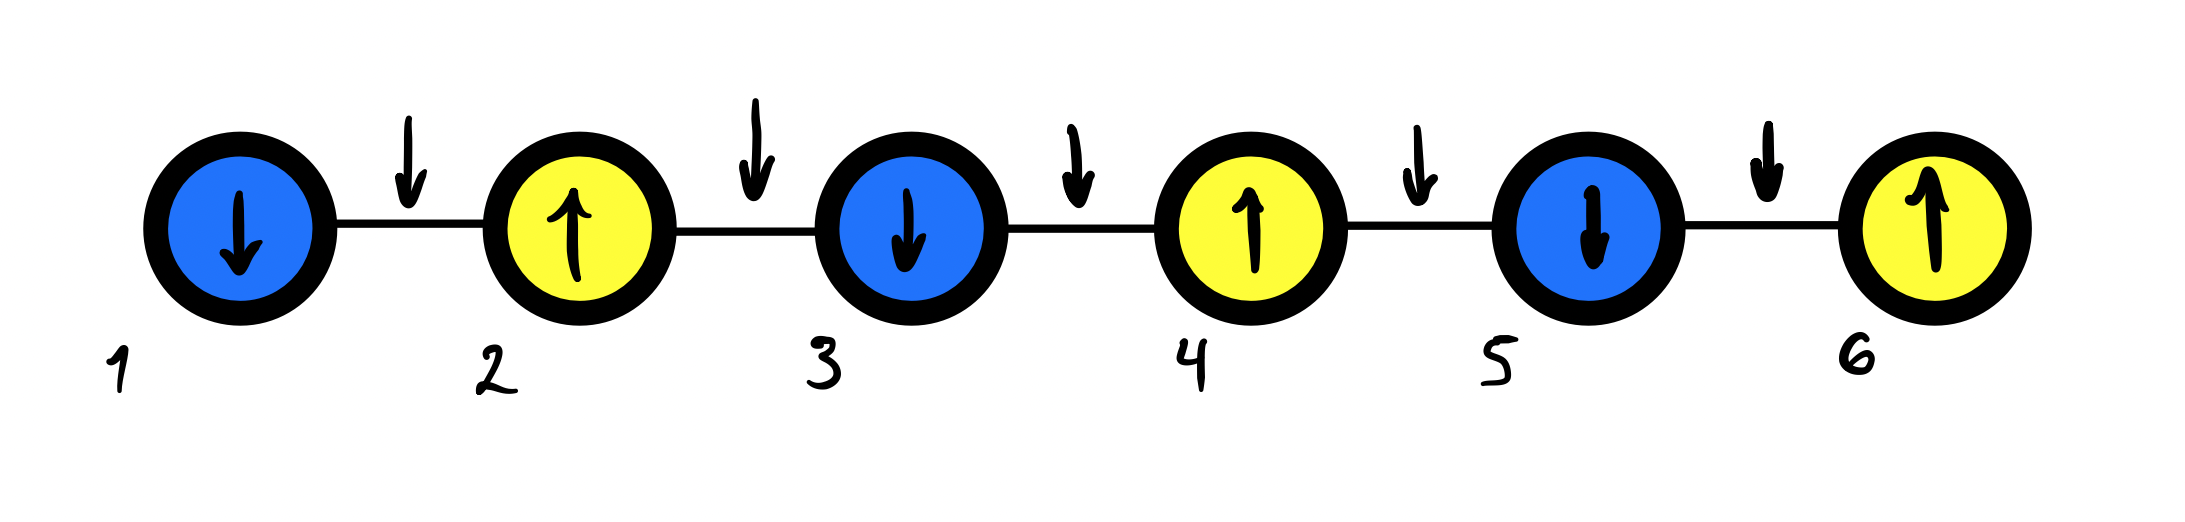
\includegraphics[width=\linewidth]{spins.png} % change jpg to pdf when doing the final compilation of the pdf
\end{subfigure}
\caption{Quantum link model with spins.\label{fig:spins}}
\end{figure}







\end{appendices}



\end{spacing}
\end{document}

%%%%%%%%%%%%%%%%%%%%%%%%%%%%%%%%%%%%%%%%%%%%%%%%%%%%%%%%%%%%%
